\documentclass[11pt]{article}
\usepackage[a4paper,margin=28mm]{geometry}
\usepackage{amsmath,amssymb,amsthm}
\usepackage{graphicx}
\usepackage{fancyhdr}
\usepackage[hidelinks]{hyperref}
\graphicspath{{./}{manuscript/}}

\hypersetup{
      pdftitle={A First-Moment-Constrained Rayleigh Problem on the Half-Line},
      pdfauthor={Davide Marchini},
      pdfsubject={A first-moment-constrained Rayleigh problem and its trend-kernel application}
}
\pagestyle{fancy}
\fancyhf{}
\lhead{Moment-constrained Rayleigh problem}
\rhead{\thepage}
\setlength{\headheight}{14pt}
\renewcommand{\headrulewidth}{0.3pt}

\newtheorem{theorem}{Theorem}[section]
\newtheorem{lemma}[theorem]{Lemma}
\newtheorem{proposition}[theorem]{Proposition}
\newtheorem{corollary}[theorem]{Corollary}
\theoremstyle{definition}
\newtheorem{definition}[theorem]{Definition}
\theoremstyle{remark}
\newtheorem{remark}[theorem]{Remark}

\newcommand{\A}{\mathcal A}
\newcommand{\Rcal}{\mathcal R}
\newcommand{\supp}{\operatorname{supp}}

\title{A First-Moment-Constrained Rayleigh Problem on the Half-Line}
\author{Davide Marchini\thanks{Corresponding author: \href{mailto:davide.marchini2@gmail.com}{\texttt{davide.marchini2@gmail.com}}}}
\date{}

\begin{document}
\maketitle

\begin{abstract}
For $L>0$, consider nonnegative probability densities $f$ on the half-line satisfying
$f(0)=0$, $\int_0^\infty f=1$, and $\int_0^\infty xf(x)\,dx=L$. The Rayleigh
quotient $\Rcal(f)=\|f'\|_2^2/\|f\|_2^2$ arises as the continuum fixed-risk
turnover objective for a linear trend-following filter with serially independent
volatility-adjusted returns. The infimum is attained by a unique density. Its
continuous representative is positive on $(0,K_L)$, vanishes beyond $K_L$, and
is linear plus trigonometric on its support. The free boundary is determined by a
unique scalar root, giving $K_L/L\approx2.40748835$ and
$L^2\Rcal(f_L)\approx2.19907193$. The proof combines the direct method, a
one-dimensional obstacle system, compression of positivity components, and scalar
free-boundary analysis. Discrete minima converge to the continuum minimum, and
interpolated near-minimizers converge to the optimizer. For finitely supported
kernels, further results identify distributional conditions under which the same
Rayleigh objective governs expected turnover; a profilewise short-memory limit is
also established.
\end{abstract}


\section{Introduction}
The design of a smooth trend-following signal can be viewed as a filter-design
problem. In a white-noise benchmark, fixing the risk of the signal and
penalizing changes in the position reduces the problem to a ratio of quadratic
energies: the numerator measures the squared first difference of the kernel,
while the denominator fixes signal variance. A further scale constraint is
needed to prevent the trivial solution obtained by making the filter
arbitrarily slow. The first moment of the kernel itself provides the natural
lookback constraint.

The main result establishes existence and uniqueness and identifies the optimizer
explicitly. The proof begins with the direct method, derives a one-dimensional
obstacle system, and uses compression of positivity components to obtain a single
compact support interval. The free-boundary equations then reduce the profile to a
linear-plus-trigonometric form determined by a unique scalar root. A
discrete-to-continuum theorem gives convergence of the scaled minima and of
interpolated near-minimizers. Further results treat finite-support distributional
extensions and the profilewise short-memory limit under their stated hypotheses.

The statements proved here are accompanied by a Lean~4 formalization with
mathlib, described in Appendix~\ref{app:lean}. In particular the main theorem,
the discrete convergence theorem, and the decimal constants printed above are
machine-checked, and the certified arithmetic of
Appendix~\ref{app:certificate} is reproduced by a script shipped with the
formalization.

A closely related variational formulation was studied by Martin~\cite{Martin2021}.
In his Section~2.2, path length is minimized under
a unit $L^2$ norm and the constraint
$\int_0^\infty t^{-1}K(t)^2\,dt=1/\tau$; EMA2$=$ solves the resulting
Euler--Lagrange equation and is optimal in that formulation. The present problem
instead imposes mass, nonnegativity, zero trace, and first moment on the kernel
density. These different constraints lead to different Euler--Lagrange and
free-boundary structures: the resulting optimizer is compactly supported, whereas
the EMA2$=$ kernel has infinite support and exponential decay.

Broad empirical work on time-series momentum and trend following provides
economic context~\cite{MoskowitzOoiPedersen,HurstOoiPedersen}, but does not
address this kernel-design theorem. Related transaction-filter and dynamic
portfolio work~\cite{BalversWu,GarleanuPedersen} optimizes returns or trading
policies under predictability and costs; EMA performance studies
~\cite{GrebenkovSerror,ZakamulinGiner} likewise differ from the fixed-risk,
fixed-lookback minimum-turnover problem. This distinction also separates the
present result from stochastic-control work such as Martin~\cite{Martin2012}.

Under a common first-moment normalization, the two objective values have ratio
approximately $0.5498$; the corresponding Gaussian expected-turnover ratio is
approximately $0.7415$. The exact calculation is given in
Section~\ref{sec:financial}.

The remaining sections prove the theorem, establish discrete convergence, and
record the distributional and serial-dependence qualifications of the extensions.
Appendices~\ref{app:discrete}--\ref{app:extensions} contain the corresponding
proofs, and Appendices~\ref{app:certificate}--\ref{app:lean} record the certified
arithmetic and the Lean~4 formalization.

\section{The variational problem}
For $L>0$, define
\[
\A_L=\left\{f\in H^1(0,\infty):
 f\geq0\ \text{a.e.},\ f(0)=0,\
 \int_0^\infty f(x)\,dx=1,\
 \int_0^\infty xf(x)\,dx=L\right\}.
\]
The value $f(0)$ is understood in the Sobolev trace sense. We study
\[
 \Lambda_L=\inf_{f\in\A_L}\Rcal(f),\qquad
 \Rcal(f)=\frac{\|f'\|_{L^2(0,\infty)}^2}{\|f\|_{L^2(0,\infty)}^2}.
\]
For $0<t<2\pi$, set
\[
 p(t)=2-t\cot\frac t2,
 \qquad
 Q(t)=t^4-6t^2p(t)+3p(t)^3\bigl(p(t)-2\bigr).
\]
As proved in Lemma~\ref{lem:branch}, $Q$ has a unique zero $t_*$ in
$(0,2\pi)$. Define
\[
 A_*:=\frac{t_*\sin t_*+\cos t_*-1}{t_*(\cos t_*-1)},
 \qquad
 C_*:=\frac{t_*\cos t_*-\sin t_*}{t_*(\cos t_*-1)}.
\]

\begin{theorem}[Existence, uniqueness, and characterization of the optimizer]\label{thm:main}
For every $L>0$, the infimum $\Lambda_L$ is attained by a unique density up
to equality almost everywhere. Its continuous representative has positivity
set $(0,K_L)$ and has the form
\[
 f_L(x)=
 \begin{cases}
 \displaystyle\frac{1}{K_L I_0}F_*\!\left(\frac{x}{K_L}\right),&0\leq x\leq K_L,\\[7pt]
 0,&x>K_L,
 \end{cases}
\]
where
\[
 F_*(y)=A_*\sin(t_*y)+C_*\bigl(\cos(t_*y)-1\bigr)+y,
\]
with
\[
 t_*\approx3.570129027812636,
\quad A_*\approx0.497710545413385,
\quad C_*\approx0.415370649651761.
\]
Writing
\[
 I_0=\int_0^1F_*(y)\,dy,
\qquad I_1=\int_0^1yF_*(y)\,dy,
\]
one obtains
\[
 \kappa_*:=\frac{K_L}{L}=\frac{I_0}{I_1}=\frac{1}{C_*}
 =\frac{t_*(\cos t_*-1)}{t_*\cos t_*-\sin t_*}
 \approx2.407488350075723,
\]
and
\[
 \Rcal(f_L)=\frac{t_*^2}{K_L^2}
 =\frac{t_*^2 C_*^2}{L^2}
 \approx\frac{2.199071934562496}{L^2}.
\]
In particular, the dimensionless minimum is
\[
 \lambda_*:=L^2\Lambda_L=t_*^2C_*^2
 \approx2.199071934562496.
\]
Equivalently, every $f\in\A_L$ satisfies
\[
 \int_0^\infty |f'|^2\,dx
 \geq \frac{t_*^2C_*^2}{L^2}\int_0^\infty f^2\,dx,
\]
with equality if and only if $f=f_L$ almost everywhere.
\end{theorem}

\begin{remark}[Proof roadmap and analytic background]\label{rem:standard-inputs}
The proof is self-contained apart from standard one-dimensional Sobolev
compactness, traces, weak lower semicontinuity, and direct-method facts
\cite{Brezis,LiebLoss}. The multiplier measure, one-dimensional obstacle
regularity, and compression argument are developed explicitly; the obstacle
framework is classical~\cite{KinderlehrerStampacchia,Friedman}, with
one-dimensional regularity as in Mandallena~\cite{Mandallena}. We also use the
standard concavity, level-set, zero-extension, area, and trapezoidal facts
needed in the proofs. Sharp Rayleigh and Poincaré context is surveyed by
Kuznetsov and Nazarov~\cite{KuznetsovNazarov}; related compactly supported Nash
extremals and variational treatments are given by Carlen--Loss
\cite{CarlenLoss} and Bouin--Dolbeault--Schmeiser~\cite{BouinDolbeaultSchmeiser}.
\end{remark}

\begin{remark}[The universal constant]
The number $\kappa_*$ is not introduced as a fitted numerical constant. It
is the unique dimensionless free-boundary/eigenvalue constant generated by the
optimization problem. Equivalently, if $x_*=t_*/2$, then
\[
 \kappa_*=
 \frac{2x_*\tan^2 x_*}
 {x_*\tan^2 x_*+\tan x_*-x_*},
\]
where $x_*$ is the unique admissible root inherited from the scalar
consistency equation $Q(t)=0$. We do not require, and do not know, an elementary closed-form representation of
$t_*$ or $\kappa_*$. The intrinsic root characterization is sufficient for the
results below.
\end{remark}

The uniqueness and numerical statements in Theorem~\ref{thm:main} are proved
in Sections~3--8 below; the theorem is stated here in advance so that its
constants and equality case are available for reference.

\section{Scaling}
By Lemma~\ref{lem:scaling} the problem at lookback $L$ reduces to the
problem at unit mean up to the explicit factor $L^{-2}$, so the unit-mean case
carries all of the content.
\begin{lemma}\label{lem:scaling}
If $g(y)=Lf(Ly)$, then $f\in\A_L$ if and only if $g\in\A_1$, and
\[
 \Rcal(f)=L^{-2}\Rcal(g).
\]
Thus $\Lambda_L=L^{-2}\Lambda_1$, and any optimal support endpoint must be proportional to $L$.
\end{lemma}
\begin{proof}
Substitute $x=Ly$ and $f(x)=L^{-1}g(x/L)$. Then
\[
 \int g=\int f=1,
 \qquad
 \int yg(y)\,dy=L^{-1}\int xf(x)\,dx=1.
\]
Moreover,
\[
 f'(x)=L^{-2}g'(x/L),
\]
so
\[
 \|f'\|_2^2=L^{-3}\|g'\|_2^2,
 \qquad
 \|f\|_2^2=L^{-1}\|g\|_2^2.
\]
Taking the quotient proves the claim.
\end{proof}

\section{Compactness issues}
\begin{lemma}[Nondegeneracy of the denominator]\label{lem:l2}
Every $f\in\A_L$ satisfies
\[
 \|f\|_2^2\geq\frac{1}{8L}.
\]
\end{lemma}
\begin{proof}
The mean constraint gives
\[
 \int_{2L}^\infty f(x)\,dx\leq\frac{1}{2L}\int_0^\infty xf(x)\,dx=\frac12.
\]
Hence $\int_0^{2L}f\geq1/2$. Cauchy--Schwarz gives
\[
 \frac14\leq\left(\int_0^{2L}f\right)^2
 \leq2L\int_0^{2L}f^2
 \leq2L\|f\|_2^2.
\]
\end{proof}

\begin{lemma}[Uniform tail control]\label{lem:tail}
Let $(f_n)$ be a nonnegative sequence in $H^1(0,\infty)$ such that
$\sup_n\|f_n'\|_2<\infty$ and
$\sup_n\int_R^\infty f_n(x)\,dx\leq\eta(R)$, where $\eta(R)\to0$ as
$R\to\infty$. Then
\[
 \sup_n\int_R^\infty f_n(x)^2\,dx\longrightarrow0
 \qquad(R\to\infty).
\]
\end{lemma}
\begin{proof}
For fixed $R$, apply the one-dimensional Gagliardo--Nirenberg inequality on
$(0,\infty)$ to the translated function $v_n(y)=f_n(R+y)$. Since
$\|v_n\|_1=\int_R^\infty f_n$ and $\|v_n'\|_2\leq\|f_n'\|_2$,
\[
 \int_R^\infty f_n^2
 \leq 2^{2/3}\left(\int_R^\infty f_n\right)^{4/3}
 \|f_n'\|_2^{2/3}.
\]
The right-hand side tends to zero uniformly in $n$ as $R\to\infty$.
\end{proof}

\begin{proposition}[Existence]\label{prop:existence}
A minimizing sequence is bounded in $H^1(0,\infty)$, is locally precompact in $L^2$ and in the uniform topology, cannot lose probability mass at infinity, and cannot lose first moment at infinity without contradicting scaling. Consequently the direct method yields a minimizer.
\end{proposition}
\begin{proof}
The class $\A_L$ is nonempty; for example,
$6x(2L-x)_+/(2L)^3$ belongs to it. Let $(f_n)\subset\A_L$ be minimizing
and choose $Q<\infty$ such that $\Rcal(f_n)\leq Q$. On any half-line,
the one-dimensional Gagliardo--Nirenberg inequality gives
\begin{equation}\label{eq:gn}
 \|v\|_2^2
 \leq 2^{2/3}\|v\|_1^{4/3}\|v'\|_2^{2/3}.
\end{equation}
Indeed, $\|v\|_2^2\leq\|v\|_1\|v\|_\infty$ and
$\|v\|_\infty^2\leq2\|v\|_2\|v'\|_2$. Since $\|f_n\|_1=1$, writing $X_n=\|f_n'\|_2$ yields
\[
 X_n^2\leq Q\|f_n\|_2^2
 \leq 2^{2/3}QX_n^{2/3}.
\]
Thus $(f_n)$ is bounded in $H^1(0,\infty)$. After taking a subsequence,
$f_n\rightharpoonup f$ in $H^1(0,\infty)$. On every bounded interval the
compact embedding $H^1\hookrightarrow C^0$ in one dimension, followed by a
diagonal argument, gives local uniform and local $L^2$ convergence. In
particular, $f\geq0$ and continuity of the trace gives $f(0)=0$.

The first moment gives tightness of probability mass:
\[
 \int_R^\infty f_n(x)\,dx\leq\frac{L}{R}.
\]
Together with local convergence, this proves $\int f=1$. Lemma~\ref{lem:tail}, together with
\[
 \int_R^\infty f_n(x)\,dx\leq\frac{L}{R},
\]
shows that the $L^2$ tails vanish uniformly. By Fatou's lemma, the same tail bound holds for the limit. Combining it with strong local $L^2$ convergence proves
$f_n\to f$ strongly in $L^2(0,\infty)$. Fatou's lemma also gives
\[
 m:=\int_0^\infty xf(x)\,dx\leq L.
\]
We have $m>0$: if $m=0$ then $xf(x)=0$ almost everywhere on $(0,\infty)$, so
$f=0$ almost everywhere there, contradicting $\int f=1$. Weak lower semicontinuity of the
Dirichlet integral and strong convergence of the denominator imply
\[
 \Rcal(f)\leq\liminf_{n\to\infty}\Rcal(f_n)=\Lambda_L.
\]

The only remaining possible defect is that a vanishing amount of mass carries nonzero first moment to infinity. If $m<L$, dilate the limit to mean $L$ by
\[
 \widetilde f(x)=\frac{m}{L}f\!\left(\frac{m}{L}x\right)
\]
to obtain an admissible density satisfying
\[
 \Rcal(\widetilde f)=\left(\frac{m}{L}\right)^2\Rcal(f)<\Rcal(f).
\]
The quotient $\Rcal(f)$ is positive: otherwise $f'=0$ almost everywhere, so
$f$ would be a constant $L^2$ function and hence would vanish, contrary to
$\int f=1$. This is the nondegeneracy of
Lemma~\ref{lem:l2} in the case $L=1$. Thus the last display is strictly below $\Lambda_L$, a
contradiction. Therefore $m=L$, $f\in\A_L$, and $f$ is a minimizer.
\end{proof}

\section{Euler--Lagrange and obstacle system}
Let $f$ be a minimizer and write
\[
 q=\Rcal(f)>0.
\]
Indeed, $f\not\equiv0$ and $f(0)=0$, so $\int_0^\infty |f'|^2>0$.

\begin{proposition}[Optimality system and local regularity]\label{prop:obstacle}
There are constants $a,b$ and a nonnegative Radon measure $\mu$, supported on the contact set $\{f=0\}$, such that
\begin{equation}\label{eq:kkt}
 -f''-qf+a+bx=\mu
\end{equation}
in distributions, with
\[
 f\geq0,
 \quad \mu\geq0,
 \quad \int f\,d\mu=0.
\]
Moreover, $\mu\in L^\infty_{\mathrm{loc}}(0,\infty)$ and
$f\in W^{2,\infty}_{\mathrm{loc}}(0,\infty)\subset C^{1,1}_{\mathrm{loc}}(0,\infty)$.
\end{proposition}
\begin{proof}
Set
\[
 \ell(h):=\int_0^\infty f'h'\,dx-q\int_0^\infty fh\,dx,
 \qquad
 M(h):=\left(\int_0^\infty h\,dx,
                 \int_0^\infty xh\,dx\right).
\]
The derivative of the quotient at $f$ is
\[
 D\Rcal(f)[h]=\frac{2}{\|f\|_2^2}\ell(h).
\]
The positivity set $\Omega=\{f>0\}$ is a nonempty open set. Choose two
nonnegative functions $\phi_1,\phi_2\in C_c^\infty(\Omega)$ whose supports lie
in small disjoint neighborhoods of two distinct points of $\Omega$. By
shrinking the supports if necessary, their mass--moment vectors
\[
 M(\phi_i)=\left(\int_0^\infty\phi_i\,dx,
                       \int_0^\infty x\phi_i\,dx\right)
\]
are linearly independent: for a bump concentrated near $x_i$, the ratio of
its first moment to its mass is arbitrarily close to $x_i$. Let
$R:\mathbb R^2\to\operatorname{span}\{\phi_1,\phi_2\}$ be the resulting
linear right inverse of $M$.

For a nonnegative test function $\psi\in C_c^\infty(0,\infty)$, put
\[
 h_\psi=\psi-R(M\psi).
\]
Then $M(h_\psi)=0$. Outside the fixed compact support of the $\phi_i$, the
negative part of $h_\psi$ vanishes; on that support, $f$ has a positive
minimum. Consequently $f+\varepsilon h_\psi\geq0$ for all sufficiently small
$\varepsilon>0$. This is an admissible one-sided variation, so minimality gives
$\ell(h_\psi)\geq0$.

The linear functional $\ell\circ R$ on $\mathbb R^2$ has the form
$(u,v)\mapsto-au-bv$ for unique constants $a,b$. Therefore
\[
 \mu(\psi):=\ell(\psi)+a\int\psi+b\int x\psi\geq0
 \qquad(\psi\in C_c^\infty,\ \psi\geq0).
\]
Thus $\mu$ is a positive distribution and hence, by the standard theorem on
positive distributions, a locally finite
nonnegative Radon measure. If $\psi$ is supported compactly in $\Omega$, then
both signs of $h_\psi$ are admissible for small parameter, so
$\mu(\psi)=0$. Hence the restriction of the positive measure $\mu$ to every
compact subset of $\Omega$ is zero, and therefore
$\operatorname{supp}\mu\subseteq\{f=0\}$, and the definition of $\ell$ gives
\eqref{eq:kkt}. Since $f$ is continuous and vanishes on the support of $\mu$,
$f=0$ $\mu$-almost everywhere, which is the stated complementarity relation.

It remains to prove the asserted regularity. We use the following elementary
one-dimensional fact. If $J$ is a bounded interval, $v\in H^1(J)$,
$\psi\in C^{1,1}(J)$, $v\geq\psi$, and the distribution $-v''$ is a
nonnegative measure supported on $\{v=\psi\}$, then
$v\in C^{1,1}_{\mathrm{loc}}(J)$. Here and below we use the continuous
representative of $v$. The distributional inequality $-v''\geq0$ implies that
this representative is concave: equivalently, $v'$ has a nonincreasing
bounded-variation representative, and integration recovers the concavity
inequality for $v$. In particular the one-sided derivatives $D^-v$ and
$D^+v$ exist at every interior point and satisfy $D^-v\geq D^+v$.

At an interior contact point $x$, the inequalities
$v(x+h)-v(x)\geq\psi(x+h)-\psi(x)$ for positive and negative $h$ give
\[
 D^+v(x)\geq\psi'(x)\geq D^-v(x).
\]
Thus all three quantities are equal, so $v$ is differentiable at every
contact point and $v'(x)=\psi'(x)$. On each component of the open set
$\{v>\psi\}$ the measure $-v''$ vanishes, so $v$ is affine there. It follows
that $v$ is differentiable at every interior point of $J$ unless the whole
interval is one free component; in that exceptional case $v$ is affine and
the conclusion is immediate.

It remains to bound the variation of its derivative. If two interior points
$x<y$ lie in the same free component, then $v'(x)=v'(y)$. Otherwise, let $r$
be $x$ when $x$ is a contact point and the right endpoint of the free
component containing $x$ otherwise. Define $s$ from $y$ analogously, using
the left endpoint of its free component. The assumption that $x$ and $y$ do
not lie in the same free component ensures that these endpoints are interior
contact points and that
$x\leq r\leq s\leq y$. Affineness on the free components and differentiability
at their contact endpoints give
$v'(x)=\psi'(r)$ and $v'(y)=\psi'(s)$. Concavity and the Lipschitz property of
$\psi'$ now give
\[
 0\leq v'(x)-v'(y)
 = \psi'(r)-\psi'(s)
 \leq \|\psi'\|_{\mathrm{Lip}}(s-r)
 \leq \|\psi'\|_{\mathrm{Lip}}(y-x).
\]
If the contact set is empty, the support assumption gives
$-v''=0$ throughout $J$, and $v$ is affine, so the same conclusion is
immediate. This proves that $v'$ is locally Lipschitz and hence that
$v\in C^{1,1}_{\mathrm{loc}}(J)$.

Now fix $J\Subset(0,\infty)$. Since one-dimensional $H^1$ functions are
continuous, $F:=qf-a-bx$ is bounded on $J$. Choose
$h\in W^{2,\infty}(J)$ with $-h''=F$ and put $v=f-h$. Equation~\eqref{eq:kkt}
becomes
\[
 -v''=\mu,
 \qquad v\geq-h,
 \qquad \operatorname{supp}\mu\subseteq\{v=-h\}.
\]
The preceding fact, with obstacle $-h$, gives
$v\in C^{1,1}_{\mathrm{loc}}(J)$ and hence
$f\in W^{2,\infty}_{\mathrm{loc}}(J)$. Finally
\eqref{eq:kkt} shows that $\mu$ has an $L^\infty_{\mathrm{loc}}$ density.
\end{proof}

On every component of the positivity set, Proposition~\ref{prop:obstacle} gives
\begin{equation}\label{eq:ode}
 f''(x)+qf(x)=a+bx.
\end{equation}

\begin{lemma}[Contact-set compression]\label{lem:compression}
Let $u\in H^1(0,\infty)$ be nonnegative, satisfy $u(0)=0$, be integrable,
and have finite first moment. Put $P=\{u>0\}$ and
\[
 T(x)=\int_0^x\mathbf1_P(s)\,ds.
\]
There is a nonnegative $g\in H^1(0,\infty)$ with $g(0)=0$ such that
\begin{equation}\label{eq:compression-invariants}
 \int g=\int u,
 \qquad \int g^2=\int u^2,
 \qquad \int |g'|^2=\int |u'|^2,
\end{equation}
and
\begin{equation}\label{eq:compression-moment}
 \int_0^\infty yg(y)\,dy
 =\int_0^\infty T(x)u(x)\,dx
 \leq\int_0^\infty xu(x)\,dx.
\end{equation}
The last inequality is strict precisely when
\[
 \int_P\bigl|P^c\cap(0,x)\bigr|u(x)\,dx>0,
\]
where $|\cdot|$ denotes Lebesgue measure; in particular, this holds whenever
the zero set has positive measure below a subset of $P$ carrying positive
$u(x)\,dx$ mass.
\end{lemma}
\begin{proof}
Use the continuous representative of $u$ and write the open set $P$ as the
disjoint union of its countably many components $I_n=(a_n,b_n)$. The endpoint
$b_n$ is allowed to be infinite. The map $T$ is absolutely continuous and
satisfies $T'=\mathbf1_P$ almost everywhere. Consequently, on $I_n$,
\[
 T(x)=T(a_n)+x-a_n,
\]
so $T$ maps $I_n$ isometrically onto
\[
 \widehat I_n:=\bigl(T(a_n),T(a_n)+b_n-a_n\bigr).
\]
These image intervals have disjoint interiors. They cover $(0,|P|)$ up to a
null set, where this interval is understood as $(0,\infty)$ if $|P|=\infty$.
Indeed, the range of the continuous nondecreasing function $T$ contains every
$y$ with $0<y<|P|$. If such a $y$ is not in any $\widehat I_n$, a point
$x$ with $T(x)=y$ must lie in $P^c$. On every bounded interval, the standard
absolute-continuity estimate
\[
 |T(E)|\leq\int_E|T'(x)|\,dx
\]
shows that $T(P^c)$ has measure zero, because $T'=0$ almost everywhere on
$P^c$. Exhausting the half-line by bounded intervals proves the asserted
coverage. It follows that, for every nonnegative measurable $\varphi$,
change of variables on the components gives the push-forward identity
\[
 \sum_n\int_{\widehat I_n}\varphi(y)\,dy
 =\int_P\varphi(T(x))\,dx
 =\int_0^{|P|}\varphi(y)\,dy.
\]

For each $n$, translate $u|_{I_n}$ to $\widehat I_n$ by
$U_n(T(x))=u(x)$ and extend it by zero outside $\widehat I_n$. At every finite
endpoint of $I_n$, continuity gives $u=0$, since the endpoint does not belong
to $P$. If $b_n=\infty$, then $u(x)\to0$ as $x\to\infty$, because a half-line
$H^1$ function is uniformly continuous and belongs to $L^2$. The standard
one-dimensional zero-extension criterion therefore gives
$U_n\in H^1(0,\infty)$, with
\[
 U_n'(T(x))=u'(x)\quad\text{for almost every }x\in I_n.
\]
The translated intervals are disjoint and every translated piece meeting the
origin has zero trace there. Thus
\[
 g_N:=\sum_{n=1}^N U_n
\]
belongs to $H^1(0,\infty)$, is nonnegative, and satisfies $g_N(0)=0$. For
$M>N$, disjointness and translation invariance give
\[
 \|g_M-g_N\|_2^2=\sum_{N<n\leq M}\int_{I_n}u^2,
 \qquad
 \|g_M'-g_N'\|_2^2=\sum_{N<n\leq M}\int_{I_n}|u'|^2.
\]
An absolutely continuous function has derivative zero almost everywhere on
each level set, so $u'=0$ almost everywhere on $P^c=\{u=0\}$. Hence the two
series on the right exhaust the full square and Dirichlet energies of $u$, and
$(g_N)$ is Cauchy in $H^1(0,\infty)$. Let $g$ be its limit. Continuity of the
trace gives $g(0)=0$, and convergence of the two norm identities gives
\[
 \int g^2=\int u^2,
 \qquad
 \int|g'|^2=\int|u'|^2.
\]

Because the $U_n$ are nonnegative and have disjoint interiors, $g_N$ increases
pointwise to the function obtained by placing all translated pieces. Its
pointwise limit agrees almost everywhere with the $H^1$ limit $g$, as follows
by taking an almost-everywhere convergent subsequence of the $L^2$-convergent
sequence. Monotone convergence, translation on each component, and the
push-forward identity now give
\[
 \int_0^\infty g(y)\,dy
 =\sum_n\int_{I_n}u(x)\,dx
 =\int_0^\infty u(x)\,dx
\]
and
\[
 \int_0^\infty yg(y)\,dy
 =\sum_n\int_{I_n}T(x)u(x)\,dx
 =\int_P T(x)u(x)\,dx
 =\int_0^\infty T(x)u(x)\,dx.
\]
The last integral is finite because $0\leq T(x)\leq x$. This proves all three
identities in~\eqref{eq:compression-invariants} and the equality in
\eqref{eq:compression-moment}.

Finally,
\[
 x-T(x)=\bigl|P^c\cap(0,x)\bigr|\geq0,
\]
and therefore
\[
 \int_0^\infty xu(x)\,dx-\int_0^\infty T(x)u(x)\,dx
 =\int_P\bigl|P^c\cap(0,x)\bigr|u(x)\,dx.
\]
This proves both the inequality and its stated strictness criterion.
\end{proof}

\begin{proposition}[Support geometry and smooth fit]\label{prop:geometry}
There is a finite $K>0$ such that $f=0$ on $(K,\infty)$, the obstacle reaction vanishes on $(0,K)$, and
\[
 f(0)=0,
 \qquad f(K)=0,
 \qquad f'(K^-)=0.
\]
Consequently equation~\eqref{eq:ode} holds throughout $(0,K)$. The scalar analysis below shows that in fact $f>0$ on $(0,K)$.
\end{proposition}
\begin{proof}
By Proposition~\ref{prop:obstacle}, $f\in C^{1,1}_{\mathrm{loc}}$ and $\mu\in L^\infty_{\mathrm{loc}}$. Apply Lemma~\ref{lem:compression} to $f$. The compressed function has the same mass, $L^2$ norm, and Dirichlet energy, hence the same Rayleigh quotient. Let $m$ denote its first moment. We have $m>0$: otherwise $yg(y)=0$ almost everywhere, so the nonnegative
function $g$ would vanish almost everywhere on $(0,\infty)$, contradicting
$\int g=1$. If $m<L$, the dilation
\[
 \widetilde g(x)=\frac{m}{L}g\left(\frac{m}{L}x\right)
\]
belongs to $\A_L$ and satisfies
$\Rcal(\widetilde g)=(m/L)^2\Rcal(f)<\Rcal(f)$, contradicting minimality.
Hence compression cannot strictly decrease the first moment. By the strictness
statement in Lemma~\ref{lem:compression}, this rules out both an initial zero
interval followed by positive mass and any positive-measure gap before
positive mass. Here is the measure argument explicitly. If the contact set
had positive measure in the interior of the convex hull of $P=\{f>0\}$, then
there would be an $R$ strictly below the right endpoint of the hull such that
$E:=P^c\cap(0,R)$ has positive measure. Since $R$ lies below that endpoint,
$P\cap(R,\infty)$ is nonempty; openness of $P$ therefore supplies a nonempty
open interval $J\subset P\cap(R,\infty)$.
For every $x\in J$ one has
$|P^c\cap(0,x)|\geq|E|$, and
$\int_J f(x)\,dx>0$. Hence
\[
 \int_P|P^c\cap(0,x)|f(x)\,dx
 \geq |E|\int_J f(x)\,dx>0,
\]
contradicting the absence of strict moment decrease. The same argument with
$E$ contained in an initial zero interval rules out a positive left endpoint
of the convex hull. Thus the convex hull of $\{f>0\}$ begins at the origin and
the contact set has measure zero inside that hull. Since
$\mu\in L^\infty_{\mathrm{loc}}$ and is supported on the contact set, it
vanishes in the interior of the hull. If that hull were unbounded,
equation~\eqref{eq:ode} would hold on all of $(0,\infty)$ and would give
\[
 f(x)=A\sin(kx)+B\cos(kx)+\frac{a}{q}+\frac{b}{q}x,
 \qquad k=\sqrt q,
\]
which cannot belong to $L^1\cap L^2$ unless it vanishes identically. Indeed,
$b\neq0$ gives linear growth. If $b=0$, then the remaining function is a
constant plus a periodic trigonometric polynomial. Its squared mean over a
period is
\[
 \frac{A^2+B^2}{2}+\left(\frac aq\right)^2,
\]
which is positive unless $A=B=a=0$; in the nonzero case its $L^2$ integral on
the half-line therefore diverges. Thus the hull is $[0,K]$ for some finite
$K$, and equation~\eqref{eq:ode} holds throughout $(0,K)$.

Continuity gives $f(K)=0$. Since
$f\in C^{1,1}_{\mathrm{loc}}(0,\infty)$ and is identically zero immediately
to the right of $K$, its derivative is continuous at the interior point $K$ and
$f'(K^-)=f'(K^+)=0$.
\end{proof}

\section{Solution on the positive interval}
Let $k=\sqrt q$. Solving~\eqref{eq:ode} on $(0,K)$ gives
\[
 f(x)=A\sin(kx)+B\cos(kx)+\frac{a}{q}+\frac{b}{q}x.
\]
The condition $f(0)=0$ permits the form
\[
 f(x)=A\sin(kx)+C\bigl(\cos(kx)-1\bigr)+Dx.
\]
Here $C=-a/q$ and $D=b/q$. The right-hand side of~\eqref{eq:ode} is bounded
on $(0,K)$, so $f''=a+bx-qf$ belongs to $L^\infty(0,K)$ and $f$ extends to
$W^{2,\infty}(0,K)$. Multiplying~\eqref{eq:ode} by $f$, integrating over
$(0,K)$, and using $f(0)=f(K)=0$ therefore gives
\[
 -\int_0^K |f'|^2+q\int_0^K f^2
 =a\int_0^K f+b\int_0^K xf.
\]
Using $q=\|f'\|_2^2/\|f\|_2^2$, compact support, and the mass and
first-moment constraints yields
\begin{equation}\label{eq:multiplier-balance}
 a+bL=0.
\end{equation}
On $(K,\infty)$, the reaction measure has density $a+bx$, so its
nonnegativity forces $b\geq0$. If $b=0$, then~\eqref{eq:multiplier-balance}
gives $a=0$, and the homogeneous equation together with
$f(0)=f(K)=f'(K^-)=0$ forces $f=0$. Therefore $D>0$.

Put
\[
 y=\frac{x}{K},
 \qquad t=kK.
\]
After dividing the profile by the positive factor $DK$, define
\begin{equation}\label{eq:F}
 F_t(y):=\frac{f(Ky)}{DK}
 =A_t\sin(ty)+C_t\bigl(\cos(ty)-1\bigr)+y.
\end{equation}
The multiplier identity therefore gives the useful relation
\begin{equation}\label{eq:C-support}
 C_t=\frac{C}{DK}=-\frac{a}{bK}=\frac{L}{K}.
\end{equation}
The free-boundary conditions are
\[
 F_t(1)=0,
 \qquad F_t'(1)=0.
\]
Solving the resulting two linear equations gives
\begin{equation}\label{eq:A}
 A_t=\frac{t\sin t+\cos t-1}{t(\cos t-1)},
\end{equation}
and
\begin{equation}\label{eq:C}
 C_t=\frac{t\cos t-\sin t}{t(\cos t-1)}.
\end{equation}
At $t=2\pi n$, $n\geq1$, the boundary equation $F_t(1)=0$ is inconsistent,
so these singular values do not produce profiles.

\section{Rayleigh self-consistency}
For a profile
\[
 f(x)=cF_t(x/K)\mathbf1_{[0,K]}(x),
\]
a change of variables gives
\[
 \int_0^K f'(x)^2\,dx
 =\frac{c^2}{K}\int_0^1F_t'(y)^2\,dy
\]
and
\[
 \int_0^K f(x)^2\,dx
 =c^2K\int_0^1F_t(y)^2\,dy.
\]
Therefore
\[
 \Rcal(f)=\frac{1}{K^2}
 \frac{\int_0^1F_t'(y)^2\,dy}{\int_0^1F_t(y)^2\,dy}.
\]
But $q=k^2=t^2/K^2$. Hence $t$ must solve
\begin{equation}\label{eq:G}
 G(t):=\int_0^1F_t'(y)^2\,dy
 -t^2\int_0^1F_t(y)^2\,dy=0.
\end{equation}
For the minimizing profile obtained above, $c=DK>0$; thus $F_t$ is
nonnegative and nonzero on $[0,1]$.
There is a useful simplification. Directly from~\eqref{eq:F},
\[
 F_t''+t^2F_t=t^2(y-C_t).
\]
Multiplication by $F_t$ and integration by parts therefore show that, with
\[
 I_0(t)=\int_0^1F_t(y)\,dy,
 \qquad I_1(t)=\int_0^1yF_t(y)\,dy,
\]
one has
\begin{equation}\label{eq:G-moment}
 G(t)=t^2\bigl(C_tI_0(t)-I_1(t)\bigr).
\end{equation}
For the minimizing profile, $I_0(t)>0$ and the mass and moment constraints give
$L/K=I_1(t)/I_0(t)$. Comparison with~\eqref{eq:C-support} therefore yields
$C_t=I_1(t)/I_0(t)$, which is equivalent to $G(t)=0$.

\begin{lemma}[Positive branch and unique consistency root]\label{lem:branch}
For every $0<t<2\pi$, the profile $F_t$ is strictly positive on $(0,1)$. No value $t>2\pi$ for which the boundary system is defined gives a nonnegative profile. Moreover, $G$ has exactly one zero in $(0,2\pi)$.
\end{lemma}
\begin{proof}
Let
\[
 \alpha(t)=\frac{t-\sin t}{1-\cos t}.
\]
Writing $s=t(1-y)$ and using the two conditions at $y=1$ gives the factorization
\begin{equation}\label{eq:F-factor}
 tF_t(y)=\bigl(\alpha(t)-\alpha(s)\bigr)(1-\cos s).
\end{equation}
The derivative of $\alpha$ has the sign of
\[
 d(t)=(1-\cos t)^2-(t-\sin t)\sin t.
\]
For $0<t<\pi$, one has $d(0)=d'(0)=0$ and $d''(t)=t\sin t>0$; for $\pi\leq t<2\pi$, positivity follows directly because $\sin t\leq0$. Thus $\alpha$ is strictly increasing on $(0,2\pi)$, and~\eqref{eq:F-factor} proves $F_t>0$ there. If $t>2\pi$, choose $y=1-2\pi/t$ in the equivalent, unfactored identity
\[
 tF_t(y)=\alpha(t)(1-\cos s)-s+\sin s;
\]
then $s=2\pi$ and $tF_t(y)=-2\pi<0$.

It remains to prove uniqueness of the root. Recall that
$p(t)=F_t'(0)=2-t\cot(t/2)$ and
$Q(t)=t^4-6t^2p(t)+3p(t)^3(p(t)-2)$.
For reproducibility, direct integration gives
\[
 I_0(t)=
 \frac{t^2(1+\cos t)-4t\sin t+4(1-\cos t)}
      {2t^2(1-\cos t)},
\]
\[
 I_1(t)=
 \frac{t(\cos t+2)-3\sin t}{6t(1-\cos t)}.
\]
Substitution in~\eqref{eq:G-moment} simplifies to
\begin{equation}\label{eq:G-Q}
 G(t)=-\frac{Q(t)}{12t^2}.
\end{equation}
For $0<t\leq\pi$, the elementary inequality
$x\cot x\leq1-x^2/3$ for $0<x\leq\pi/2$ gives
$p(t)\geq t^2/6$, while $p(t)\leq2$. For completeness, after multiplying by
$\sin x>0$, the inequality is equivalent to
\[
 H(x):=(1-x^2/3)\sin x-x\cos x\geq0.
\]
Here $H(0)=0$ and
$H'(x)=\frac{x}{3}(\sin x-x\cos x)>0$ for $x>0$, since
$(\sin x-x\cos x)'=x\sin x>0$. Thus the cotangent inequality is strict
for $x>0$, and hence $p(t)>t^2/6$. Therefore
\[
 t^4-6t^2p(t)<0,
 \qquad
 3p(t)^3(p(t)-2)\leq0,
\]
which proves $Q(t)<0$ on this interval.

For $\pi<t\leq\sqrt{12}$, write
\[
 u=p-2=-t\cot\frac t2=t\tan\frac{t-\pi}{2}.
\]
Here $0<u<3/5$: indeed, the elementary bounds $\pi>3.14$ and
$\sqrt{12}<3.47$ give $(t-\pi)/2<1/6$, while
$\sin x\leq x$ and $\cos x\geq1-x^2/2$ give
$u<(7/2)(12/71)<3/5$. Consequently
\[
 Q=t^2(t^2-12)
 +u\bigl(3u^3+18u^2+36u+24-6t^2\bigr)<0,
\]
because the polynomial in the bracket before $-6t^2$ is at most
$6591/125<54<6t^2$.

Finally, differentiation gives
\[
 p'(t)=\frac{t^2+p^2-2p}{2t}.
\]
For $\sqrt{12}\leq t<2\pi$, substitution of $p=2+u$ yields
\[
 Q'(t)=\frac{1}{t}\Bigl(
 t^2(t^2-12)+6t^2u^3+24t^2u^2+18t^2u
 +6u^5+39u^4+90u^3+84u^2+24u
 \Bigr)>0.
\]
Since $p(t)=2-t\cot(t/2)\to\infty$ as $t\uparrow2\pi$, the leading term
$3p(t)^4$ shows that $Q(t)\to\infty$. Together with
$Q(\sqrt{12})<0$ and the strict monotonicity above, this gives exactly one
zero $t_*\in(\sqrt{12},2\pi)$. Equation~\eqref{eq:G-Q} completes the proof.
\end{proof}

The identities relating $G$ and $Q$ are exact algebraic identities, not numerical approximations. In particular, direct differentiation gives
\[
 p'(t)=\frac{t^2+p(t)^2-2p(t)}{2t},
\]
and substitution into $Q'$ produces the displayed expression after writing $p=2+u$. Likewise, substituting the closed forms for $A_t$ and $C_t$ into $G$ gives $G(t)=-Q(t)/(12t^2)$. The interval calculation below is therefore used only to certify the decimal representation of the unique root, not to establish uniqueness.

Directed-rounding interval evaluation gives
\[
 Q(3.570129027812636)<0
 <Q(3.570129027812637),
\]
so
\[
 t_*\approx3.570129027812636.
\]
Equations~\eqref{eq:A} and~\eqref{eq:C} then give
\[
 A_*\approx0.497710545413385,
 \qquad
 C_*\approx0.415370649651761.
\]
Lemma~\ref{lem:branch} also completes the proof that every minimizer has positivity set $(0,K)$.

\section{Mass, mean, and support}
Define
\[
 I_0=\int_0^1F_*(y)\,dy,
 \qquad
 I_1=\int_0^1yF_*(y)\,dy.
\]
For
\[
 f_L(x)=cF_*\!\left(\frac{x}{K}\right)\mathbf1_{[0,K]}(x),
\]
normalization gives
\[
 cKI_0=1,
\]
and the mean condition gives
\[
 cK^2I_1=L.
\]
Consequently,
\[
 c=\frac{1}{KI_0},
 \qquad
 K=L\frac{I_0}{I_1}.
\]
By~\eqref{eq:G-moment}, $I_1/I_0=C_*$, so the equivalent identity
\begin{equation}\label{eq:support-C}
 \frac{K}{L}=\frac{1}{C_*}
\end{equation}
provides an independent check on the support calculation.
Numerically,
\[
 I_0\approx0.302496116691908,
 \qquad
 I_1\approx0.125648008507453,
\]
so
\[
 \frac{K}{L}\approx2.407488350075723.
\]
Finally,
\[
 \Rcal(f_L)=\frac{t_*^2}{K^2}
 =\frac{1}{L^2}\frac{t_*^2}{(I_0/I_1)^2}
 \approx\frac{2.199071934562496}{L^2}.
\]
Proposition~\ref{prop:existence} supplies a minimizer, and
Proposition~\ref{prop:geometry} supplies the support interval $[0,K]$ and the
endpoint identities. The preceding argument shows that every minimizer has the same value $t_*$ and hence the same dimensionless profile $F_*$. The mass and mean equations then determine $c$ and $K$ uniquely. This proves Theorem~\ref{thm:main}.

The optimizer has the scale-free representation
\[
 \Phi(z):=Lf_L(Lz)
 =\frac{1}{\kappa I_0}F_*\!\left(\frac{z}{\kappa}\right)
  \mathbf1_{[0,\kappa]}(z),
 \qquad \kappa=\frac{K_L}{L}.
\]
Thus $\Phi$ is independent of $L$, with $\int\Phi=1$ and
$\int z\Phi(z)\,dz=1$. Figure~\ref{fig:kernel} shows this universal kernel.

\begin{figure}[htbp]
 \centering
 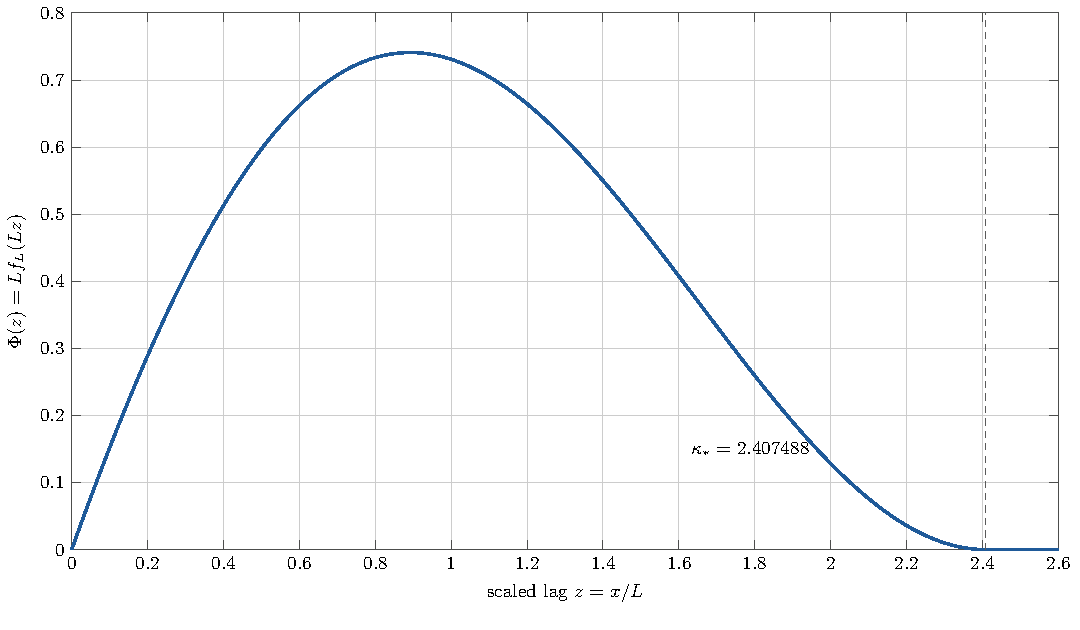
\includegraphics[width=0.82\textwidth]{rayleigh_kernel_profile.pdf}
 \caption{The universal optimal kernel in scaled coordinates. The curve is
 $\Phi(z)=Lf_L(Lz)$, and its support ends at
 $\kappa=K_L/L\approx2.407488350075723$.}
 \label{fig:kernel}
\end{figure}

\section{Endpoint behavior}
At the origin,
\[
 F_*(0)=0,
 \qquad
 F_*'(0)=1+t_*A_*>0,
 \qquad F_*'(0)\approx2.7768908656,
\]
so
\[
 f_L(x)\sim c_0x
 \qquad(x\downarrow0).
\]
At the free boundary,
\[
 F_*(1)=F_*'(1)=0,
 \qquad
 F_*''(1)>0,
 \qquad F_*''(1)\approx7.4515812118,
\]
so Taylor expansion gives
\[
f_L(x)\sim c_K(K_L-x)^2
 \qquad(x\uparrow K_L).
\]
Thus the exact endpoint powers match those of a beta density proportional to
$x^{2-1}(K_L-x)^{3-1}$, although the interior profile is not exactly beta.

\section{Financial interpretation of the Rayleigh quotient}\label{sec:financial}
Let $(r_t)_{t\in\mathbb Z}$ be centered, jointly Gaussian,
volatility-adjusted returns satisfying
\[
 \mathbb E[r_t r_s]=\delta_{ts}.
\]
Thus the returns have unit variance and are serially uncorrelated; joint
Gaussianity also makes them independent. For a nonzero square-summable sequence
of lookback weights $(w_j)_{j\geq0}$ with square-summable first difference, define
the discrete trend signal
\[
 S_t=\sum_{j\geq0}w_jr_{t-j}.
\]
The series is understood as an $L^2$ limit; square summability and white
covariance make it well defined. The same interpretation justifies the
reindexing below and passage from finite partial sums to the displayed variance
identities.
Uncorrelatedness gives
\[
 \operatorname{Var}(S_t)=\sum_{j\geq0}w_j^2.
\]

Set $w_{-1}=0$ (and extend a finitely supported kernel by zero past its
endpoint). A
reindexing of $S_{t-1}$ gives
\[
 S_t-S_{t-1}
 =\sum_{j\geq0}(w_j-w_{j-1})r_{t-j},
\]
and therefore
\[
 \operatorname{Var}(S_t-S_{t-1})
 =\sum_{j\geq0}(w_j-w_{j-1})^2.
\]

To compare kernels at the same signal risk, let
\[
 P_t=\gamma S_t,
 \qquad
 \gamma=\frac{\sigma_{\mathrm{sig}}}
 {\bigl(\sum_jw_j^2\bigr)^{1/2}},
\]
so that $\operatorname{Var}(P_t)=\sigma_{\mathrm{sig}}^2$. The one-period
position change $\Delta P_t=P_t-P_{t-1}$ is centered Gaussian with variance
\[
 \operatorname{Var}(\Delta P_t)
 =\sigma_{\mathrm{sig}}^2
 \frac{\sum_j(w_j-w_{j-1})^2}{\sum_jw_j^2}.
\]
For $Z\sim N(0,\tau^2)$, one has
$\mathbb E|Z|=\sqrt{2/\pi}\,\tau$. Hence expected absolute turnover is
\begin{equation}\label{eq:expected-turnover}
 \mathbb E|\Delta P_t|
 =\sigma_{\mathrm{sig}}\sqrt{\frac{2}{\pi}}
 \left(
 \frac{\sum_{j\geq0}(w_j-w_{j-1})^2}
      {\sum_{j\geq0}w_j^2}
 \right)^{1/2}.
\end{equation}
Any convention that reports one-way turnover as one half of the absolute
position change only alters the prefactor. Since the square root is strictly
increasing and every other factor in~\eqref{eq:expected-turnover} is fixed,
minimizing expected turnover is exactly equivalent to minimizing the discrete
Rayleigh quotient
\[
 \Rcal_{\mathrm d}(w)
 :=\frac{\sum_j(w_j-w_{j-1})^2}{\sum_jw_j^2}.
\]
Thus fixed-risk rescaling is already captured by the denominator, and $\gamma$
does not need to be carried as an additional optimization variable.

The discrete-to-continuum result provides liminf, recovery, value convergence,
and convergence of interpolated near-minimizers to the continuum optimizer; see
Theorem~\ref{thm:discrete-continuum} in Appendix~\ref{app:discrete}.

\subsection{EMA2 under first-moment normalization}
The continuous-time EMA2$=$ kernel emphasized by Martin~\cite{Martin2021} has
density proportional to $x e^{-\alpha x}$. Under the present normalization
\[
\int_0^\infty f(x)\,dx=1,
\qquad
\int_0^\infty x f(x)\,dx=L,
\]
it becomes
\[
 f_{\mathrm{EMA2}}(x)=\frac{4x}{L^2}e^{-2x/L}.
\]
Its Rayleigh quotient is
\[
 \Rcal(f_{\mathrm{EMA2}})=\frac{4}{L^2}.
\]
Under the shared first-moment normalization, the ratio of the present objective
to the EMA2$=$ objective is
\[
 \frac{\Rcal(f_L)}{\Rcal(f_{\mathrm{EMA2}})}
 =\frac{2.199071934562496}{4}
 \approx0.5497679836.
\]
Thus the Rayleigh-value ratio is approximately $0.5497679836$, and the
corresponding Gaussian expected-turnover ratio is its square root, approximately
$0.7414634068$. Equivalently, the relative differences are $45.02\%$ and
$25.85\%$, respectively. These numbers compare the kernels after a common
normalization; the underlying variational constraints remain different.

The support geometry is also different. The EMA2$=$ kernel has infinite support,
whereas the optimizer derived here satisfies $f_L(x)=0$ for $x>K_L$, where
\[
 K_L=\kappa_*L,\qquad \kappa_*\approx2.40748835.
\]

\section{Extensions and scope}\label{sec:extensions}
The exact finite-support projection-scale result gives the same minimizers for
strictly increasing aggregate costs, while turnover-isotropic inputs give exact
invariance for absolute turnover; see Propositions~\ref{prop:general-cost-invariance},
\ref{prop:exact-invariance}, and~\ref{prop:power-cost}. Correlated elliptical inputs lead instead to
the generalized quotient~\eqref{eq:correlated-turnover} of
Proposition~\ref{prop:generalized-rayleigh}, and absolutely summable
short-memory covariance has the same continuum functional profilewise, as in
Proposition~\ref{prop:short-memory}. A uniform kurtosis bound gives the stated
approximation guarantee, as in Proposition~\ref{prop:kurtosis}, and the diffuse-kernel CLT gives asymptotic Gaussian
turnover under its stated diffuseness and finite-third-moment assumptions.

These conclusions are finite-cutoff, finite-row, or profilewise as applicable;
they do not assert a general infinite-process result or convergence of
correlated minimizers, and the tilted-Gaussian example in the appendix is
deliberately nonstationary. The complete
definitions, examples, propositions, proofs, and qualifications appear in
Appendix~\ref{app:extensions}.

\section{Conclusion}
This problem is a constrained Dirichlet Rayleigh quotient with a positivity
obstacle. The direct method gives existence, the obstacle system and compression
argument yield the single compact support interval, and scalar free-boundary
analysis identifies the unique optimizer as linear plus trigonometric on
$[0,K_L]$, with
\[
 \begin{aligned}
 K_L&=\kappa_*L,\\
 \kappa_*&\approx2.407488350075723,
 \end{aligned}
\]
and
\[
 L^2\Rcal(f_L)=2.199071934562496.
\]
The universal constant has an intrinsic scalar-root characterization, with no
required elementary closed form, and determines the minimum turnover intensity
through $L^2\Rcal(f_L)=t_*^2/\kappa_*^2$.

The discrete-to-continuum theorem gives convergence of the scaled minima and of
interpolated near-minimizers. The finite-support, distributional, correlated, and
discrete conclusions retain the qualifications summarized in
Section~\ref{sec:extensions} and proved in Appendices~\ref{app:discrete}--
\ref{app:extensions}. For reference, the EMA2$=$ kernel studied in~\cite{Martin2021}
has value $4/L^2$ under the same first-moment normalization, while arising from a
different variational constraint.

\appendix
\section{Discrete-to-continuum convergence}\label{app:discrete}
We now make the discrete-to-continuum passage precise. For $h>0$, let
$\mathcal A_{h,L}$ denote the class of nonnegative sequences
$w=(w_j)_{j\geq0}$ satisfying
\[
 w\in\ell^1\cap\ell^2,
 \qquad
 Dw\in\ell^2,
 \qquad
 \sum_{j\geq0}w_j=1,
 \qquad
 h\sum_{j\geq0}j w_j=L,
\]
where $w_{-1}=0$ and $(Dw)_j=w_j-w_{j-1}$. Define
\[
 \Rcal_{\mathrm d,h}(w)
 :=\frac{\|Dw\|_2^2}{\|w\|_2^2}.
\]
The numerator and denominator are finite on this class, and the denominator is
positive because the weights have unit mass. The natural continuum scaling is
$h^{-2}\Rcal_{\mathrm d,h}$.

For a function $v$ on $[-h,\infty)$ with nonzero square norm, write
\[
 \widehat\Rcal_h(v):=
 \frac{\displaystyle\int_{-h}^{\infty}|v'(x)|^2\,dx}
      {\displaystyle\int_{-h}^{\infty}v(x)^2\,dx}.
\]
This auxiliary quotient is taken over the full interpolation domain; it is
distinct from $\Rcal$, whose domain is $(0,\infty)$.

\begin{lemma}[Piecewise-linear interpolation identities]\label{lem:discrete-interpolation}
For $w\in\mathcal A_{h,L}$, let $I_hw$ be the continuous piecewise-linear
function on $[-h,\infty)$ defined by
\[
 I_hw(-h)=0,
 \qquad
 I_hw(jh)=\frac{w_j}{h},\quad j\geq0,
\]
and, for general $w$, define $I_hw$ by linear interpolation on every mesh
interval $[jh,(j+1)h]$, using the nodal values $w_j/h$. Since $w_j\to0$,
this interpolation has limit zero at infinity. Then
$I_hw\geq0$ and
\begin{align}
 \int_{-h}^{\infty} I_hw(x)\,dx&=1,\label{eq:interp-mass}\\
 \int_{-h}^{\infty} xI_hw(x)\,dx&=L,\label{eq:interp-moment}\\
 \int_{-h}^{\infty}|(I_hw)'(x)|^2\,dx
 &=\frac{1}{h^3}\sum_{j\geq0}(w_j-w_{j-1})^2.\label{eq:interp-energy}
\end{align}
Moreover, if $S_h=\sum_jw_j^2$ and $N_h=\sum_j(w_j-w_{j-1})^2$, then
\begin{equation}\label{eq:interp-l2}
 \int_{-h}^{\infty}I_hw(x)^2\,dx
 =\frac{S_h}{h}-\frac{N_h}{6h}
 =\frac{S_h}{h}\left(1-\frac{\Rcal_{\mathrm d,h}(w)}6\right).
\end{equation}
Consequently,
\begin{equation}\label{eq:interp-quotient}
 \widehat\Rcal_h(I_hw)
 =\frac{h^{-2}\Rcal_{\mathrm d,h}(w)}
         {1-\Rcal_{\mathrm d,h}(w)/6}.
\end{equation}
\end{lemma}

\begin{proof}
The function $I_hw$ is the linear interpolant through the nodal values
$w_j/h$, with a zero node at $-h$. The hat function associated with the node
$jh$ has area $h$ and first moment $jh^2$; summing these contributions gives
\eqref{eq:interp-mass} and \eqref{eq:interp-moment}. On every mesh interval,
the derivative is constant, so \eqref{eq:interp-energy} follows directly.
For the $L^2$ norm, integration of the square of a linear function gives
\[
 3h\int I_hw^2
 =2S_h+\sum_{j\geq0}w_jw_{j+1}.
\]
Since $w\in\ell^2$ and $w_j\to0$, summation by parts gives
\[
 N_h=2S_h-2\sum_{j\geq0}w_jw_{j+1},
\]
we obtain \eqref{eq:interp-l2}, and then \eqref{eq:interp-quotient}.
\end{proof}

\begin{lemma}[Discrete recovery sequence]\label{lem:discrete-recovery}
Let $f_L$ be the continuum optimizer from Theorem~\ref{thm:main}. There exists,
for all sufficiently small $h>0$, a sequence $w^{(h)}\in\mathcal A_{h,L}$ such that
\[
 h^{-2}\Rcal_{\mathrm d,h}(w^{(h)})\longrightarrow\Rcal(f_L).
\]
\end{lemma}

\begin{proof}
Sample $f_L$ on the grid by $v_j^{(h)}=h f_L(jh)$. Since $f_L$ is compactly
supported, is $C^2$ on $[0,K_L]$, and satisfies
$f_L(0)=f_L(K_L)=f_L'(K_L)=0$, the function on $[0,\infty)$ obtained by
setting $f_L$ equal to zero past $K_L$ is $C^{1,1}$ and has a bounded weak
second derivative; a jump in the classical second derivative at $K_L$ is
harmless. The composite trapezoidal estimate for
$W^{2,\infty}$ functions, applied also to $x f_L(x)$, therefore gives
\[
 \sum_jv_j^{(h)}=1+O(h^2),\qquad
 h\sum_jjv_j^{(h)}=L+O(h^2).
\]
The difference-quotient and Riemann-sum limits also give
$h^{-2}\Rcal_{\mathrm d,h}(v^{(h)})\to\Rcal(f_L)$. Choose two nonnegative
$C_c^2$ functions $b_1,b_2$ supported in a common compact subinterval of
$(0,K_L)$ whose mass--moment vectors are linearly independent. Put
\[
 B_h=\begin{pmatrix}
 h\sum_jb_1(jh)&h\sum_jb_2(jh)\\
 h^2\sum_jj b_1(jh)&h^2\sum_jj b_2(jh)
 \end{pmatrix},
 \qquad
 d_h=\begin{pmatrix}
 1-\sum_jv_j^{(h)}\\[2pt]
 L-h\sum_jjv_j^{(h)}
 \end{pmatrix}.
\]
 The matrices $B_h$ converge to the nonsingular matrix with columns
 $(\int b_i,\int xb_i)^T$. They are therefore invertible for all sufficiently
 small $h$, with uniformly bounded inverses. The constraint defect of
 $v^{(h)}$ is $O(h^2)$, so the coefficients
$c^{(h)}=B_h^{-1}d_h=O(h^2)$. Defining
\[
 w_j^{(h)}=v_j^{(h)}+h\sum_{i=1}^2 c_i^{(h)}b_i(jh)
\]
then satisfies both discrete constraints exactly. Because $f_L$ is strictly
positive on the common compact support of the bumps, the correction preserves
nonnegativity for sufficiently small $h$.

There are $O(h^{-1})$ nonzero corrected entries. The correction has size
$O(h^3)$ per entry and first differences of size $O(h^4)$; hence its squared
$\ell^2$ norm is $O(h^5)$ and the squared norm of its first difference is
$O(h^7)$. On the other hand,
\[
 \|v^{(h)}\|_2^2=h\int f_L^2+o(h),
 \qquad
 \|Dv^{(h)}\|_2^2=h^3\int |f_L'|^2+o(h^3).
\]
Cauchy--Schwarz controls the two cross terms: the denominator changes by
$O(h^3)=o(h)$ and the numerator by $O(h^5)=o(h^3)$. Therefore
$h^{-2}\Rcal_{\mathrm d,h}(w^{(h)})\to\Rcal(f_L)$.
\end{proof}

\begin{lemma}[Discrete limsup]\label{lem:discrete-limsup}
With $\mathcal A_{h,L}$ as above,
\[
 \limsup_{h\downarrow0}\inf_{w\in\mathcal A_{h,L}}
 h^{-2}\Rcal_{\mathrm d,h}(w)\leq\Lambda_L.
\]
\end{lemma}
\begin{proof}
Apply Lemma~\ref{lem:discrete-recovery} to the continuum optimizer $f_L$.
\end{proof}

\begin{theorem}[Discrete-to-continuum convergence]
\label{thm:discrete-continuum}
Let $h_n\downarrow0$, and let $w^{(n)}\in\mathcal A_{h_n,L}$ be any sequence of
$\varepsilon_n$-minimizers, with $\varepsilon_n\to0$, in the sense that
\[
 h_n^{-2}\Rcal_{\mathrm d,h_n}(w^{(n)})
 \leq \inf_{w\in\mathcal A_{h_n,L}}
       h_n^{-2}\Rcal_{\mathrm d,h_n}(w)+\varepsilon_n.
\]
Let $f_n=I_{h_n}w^{(n)}$. On $[-h_n,0]$ the interpolant is linear, so
\[
 \int_{-h_n}^0 f_n=\frac{w^{(n)}_0}{2},
 \qquad
 \int_{-h_n}^0 x f_n(x)\,dx=-\frac{h_n w^{(n)}_0}{6}.
\]
The energy bound below implies $w^{(n)}_0/h_n=f_n(0)=O(h_n^{1/2})$, so both
quantities tend to zero. The restrictions to $[0,\infty)$ are relatively
compact for strong convergence in $L^2(0,\infty)$ and locally uniform
convergence on $[0,\infty)$. Every limit $f$ obtained in these two topologies
belongs to $\mathcal A_L$ and satisfies
\[
 \Rcal(f)\leq\liminf_{k\to\infty}
 h_{n_k}^{-2}\Rcal_{\mathrm d,h_{n_k}}(w^{(n_k)}).
\]
Moreover, if $f_L$ is the unique minimizer from Theorem~\ref{thm:main}, then
\[
 \lim_{n\to\infty}
 \inf_{w\in\mathcal A_{h_n,L}}
 h_n^{-2}\Rcal_{\mathrm d,h_n}(w)
 =\Rcal(f_L),
\]
and every sequence of discrete near-minimizers satisfies
\[
 I_{h_n}w^{(n)}\longrightarrow f_L
 \quad\text{strongly in }L^2(0,\infty)
 \quad\text{and locally uniformly on }[0,\infty).
\]
After zero extension below $-h_n$, the same sequence converges weakly to the
zero extension of $f_L$ in $H^1(\mathbb R)$.
\end{theorem}

\begin{proof}
By Lemma~\ref{lem:discrete-limsup}, every sequence of $\varepsilon_n$-minimizers
satisfies
\[
 \limsup_{n\to\infty}h_n^{-2}\Rcal_{\mathrm d,h_n}(w^{(n)})\leq\Lambda_L.
\]
Fix an arbitrary subsequence. After first passing to a further subsequence on
which the scaled quotients attain their liminf, extract the compact subsequence
constructed below and relabel it by $n$.
First note that the discrete difference operator satisfies
$N_h\leq4S_h$, hence $\Rcal_{\mathrm d,h}\leq4$. The limsup bound above
shows that $h_n^{-2}\Rcal_{\mathrm d,h_n}(w^{(n)})$ is bounded. By
Lemma~\ref{lem:discrete-interpolation},
\[
 \widehat\Rcal_h(I_h w)
 =\frac{h^{-2}\Rcal_{\mathrm d,h}(w)}
         {1-\Rcal_{\mathrm d,h}(w)/6}
\]
is uniformly bounded. Since $\|I_hw\|_1=1$, the one-dimensional
Gagliardo--Nirenberg inequality therefore gives a uniform bound on
$\|I_hw\|_{H^1(-h,\infty)}$. Indeed, writing $E=\|(I_hw)'\|_2^2$ and
$D=\|I_hw\|_2^2$, one has $D\leq C E^{1/3}$ and $E\leq C D$, hence $E$ and
$D$ are both bounded.

In particular,
\[
 |I_hw(0)|^2
 \leq h\int_{-h}^0 |(I_hw)'(x)|^2\,dx
 \leq hE\longrightarrow0,
\]
so every local uniform limit has trace zero at the origin. Weak compactness in
$H^1(\mathbb R)$, after extending each interpolant by zero on
$(-\infty,-h)$, and the one-dimensional compact embedding on bounded
intervals give a subsequence converging weakly in $H^1(\mathbb R)$ and
uniformly on compact sets. The positive-half-line first moment is
\[
 \int_0^\infty xI_hw(x)\,dx=L+\frac{hw_0}{6}.
\]
Consequently, for every $R>0$, nonnegativity implies the corrected estimate
\[
 \int_R^\infty I_hw(x)\,dx
 \leq\frac{L+hw_0/6}{R}.
\]
Lemma~\ref{lem:tail}, applied to the translated interpolants, gives a
uniformly vanishing $L^2$ tail as $R\to\infty$. Thus the convergence is strong
in $L^2(0,\infty)$, and the mass constraint passes to the limit. Fatou's lemma
also gives
\[
 m:=\int_0^\infty xf(x)\,dx\leq L.
\]
As in the existence proof, the fact that $f$ has mass one implies $m>0$.
The same argument shows that $\Rcal(f)>0$: otherwise $f'=0$ almost
everywhere, and the $L^2$ function $f$ would be a vanishing constant,
contradicting its unit mass.
The negative interpolation strip also vanishes in $L^2$: linearity there and
the estimate at the origin give
\[
 \int_{-h}^0(I_hw)^2\,dx
 =\frac h3|I_hw(0)|^2
 \leq\frac{h^2}{3}E\longrightarrow0.
\]
Hence the zero extensions in fact converge strongly in $L^2(\mathbb R)$.
Weak lower semicontinuity of the full-line Dirichlet energy and strong
convergence of the $L^2$ norm give
\[
 \Rcal(f)\leq\liminf_n\widehat\Rcal_{h_n}(I_{h_n}w^{(n)}).
\]
Indeed, the zero extensions converge weakly in $H^1(\mathbb R)$ and their
limit vanishes on $(-\infty,0)$, so its full-line quotient is exactly
$\Rcal(f)$.
Since $\Rcal_{\mathrm d,h_n}(w^{(n)})=O(h_n^2)$,
\eqref{eq:interp-quotient} implies
\[
 \widehat\Rcal_{h_n}(I_{h_n}w^{(n)})
 =h_n^{-2}\Rcal_{\mathrm d,h_n}(w^{(n)})(1+o(1)).
\]
In particular,
\[
 \Rcal(f)\leq\liminf_n
 h_n^{-2}\Rcal_{\mathrm d,h_n}(w^{(n)}).
\]
If $m<L$, the dilation
\[
 \widetilde f(x)=\frac{m}{L}f\!\left(\frac{m}{L}x\right)
\]
belongs to $\mathcal A_L$ and satisfies
$\Rcal(\widetilde f)=(m/L)^2\Rcal(f)<\Rcal(f)$. But
\[
 \Rcal(f)\leq\liminf_n h_n^{-2}\Rcal_{\mathrm d,h_n}(w^{(n)})
 \leq\limsup_n h_n^{-2}\Rcal_{\mathrm d,h_n}(w^{(n)})
 \leq\Lambda_L,
\]
while $\widetilde f\in\mathcal A_L$ implies
$\Rcal(\widetilde f)\geq\Lambda_L$, a contradiction. Hence $m=L$ and
$f\in\mathcal A_L$.
This also proves the liminf statement.

Since the initial subsequence was arbitrary, the preceding argument proves
relative compactness and the asserted liminf inequality for every
subsequential limit. Together with Lemma~\ref{lem:discrete-limsup}, it gives
\[
 \lim_{n\to\infty}\inf_{w\in\mathcal A_{h_n,L}}
 h_n^{-2}\Rcal_{\mathrm d,h_n}(w)=\Lambda_L.
\]
Every subsequential limit of discrete near-minimizers is therefore a minimizer of
$\Rcal$ on $\mathcal A_L$. Uniqueness in Theorem~\ref{thm:main} forces the limit
to be $f_L$. Relative compactness then implies convergence of the full sequence:
otherwise a subsequence staying a fixed positive distance from $f_L$ in one of
the asserted strong topologies would have a further subsequence converging to
$f_L$. Weak $H^1(\mathbb R)$ convergence of the full zero-extended sequence
follows as well: every subsequence has a further weakly convergent subsequence,
and the argument above identifies every such weak limit with the zero extension
of $f_L$.
\end{proof}

This theorem gives the liminf, recovery, value-convergence, and near-minimizer
conclusions needed to identify the compactly supported continuum kernel as the
asymptotic shape on increasingly fine half-line grids. No attainment assertion
for a fixed infinite half-line grid is needed here.


\section{Distributional and dependence extensions}\label{app:extensions}
The derivation in Section~\ref{sec:financial} separates the two probabilistic facts
that are needed: a quadratic identity for signal risk and a first absolute
moment identity for turnover. This permits an exact characterization that is
strictly broader than Gaussianity.

Unless explicitly stated otherwise, the exact non-Gaussian results in this
section concern finitely supported coefficient vectors and kernels. This is
the natural scope of the projection assumptions below and avoids silently
passing distributional identities to infinite random series. The opening
Gaussian calculation, by contrast, also covers square-summable kernels through
$L^2$ convergence.

For a finitely supported real sequence $a=(a_j)_{j\geq0}$, write
\[
 X_t(a)=\sum_{j\geq0}a_jr_{t-j},
 \qquad \|a\|_2^2=\sum_{j\geq0}a_j^2.
\]

\begin{definition}[Projection-scale white input]\label{def:projection-scale}
A centered input sequence is projection-scale white if there exist
$\sigma_r>0$ and a centered random variable $Z$, with $\mathbb E Z^2=1$, such
that for every finitely supported $a$ and every $t$,
\begin{equation}\label{eq:projection-scale}
 X_t(a)\ \overset{d}=\ \sigma_r\|a\|_2 Z.
\end{equation}
\end{definition}

Taking second moments in~\eqref{eq:projection-scale} gives
\[
 \mathbb E[X_t(a)^2]=\sigma_r^2\|a\|_2^2.
\]
By polarization, the returns are homoskedastic with variance $\sigma_r^2$
and uncorrelated across time. The converse is false: white covariance fixes
second moments but not the distribution of arbitrary linear projections.

\begin{proposition}[General aggregate-cost invariance]
\label{prop:general-cost-invariance}
Assume Definition~\ref{def:projection-scale}. Let
$c:[0,\infty)\to[0,\infty)$ be Borel and nondecreasing, with the expectations
below finite, and let $w$ be a nonzero, finitely supported kernel. Define the
cost of the net aggregate trade by
\[
 C_t=c(|P_t-P_{t-1}|).
\]
After normalizing signal variance to $\sigma_{\mathrm{sig}}^2$,
\begin{equation}\label{eq:general-cost-invariance}
 \mathbb E C_t
 =\Psi_c\!\left(\Rcal_{\mathrm d}(w)\right),
 \qquad
 \Psi_c(q):=\mathbb E\!
 \left[c\!\left(\sigma_{\mathrm{sig}}\sqrt q\,|Z|\right)\right].
\end{equation}
The function $\Psi_c$ is nondecreasing. Hence every minimizer of
$\Rcal_{\mathrm d}$ minimizes expected cost. If $c$ is strictly increasing
and $\mathbb P(|Z|>0)>0$, then $\Psi_c$ is strictly increasing and the two
problems have exactly the same minimizers.
\end{proposition}
\begin{proof}
Equation~\eqref{eq:projection-scale} gives
$\operatorname{Var}(S_t)=\sigma_r^2\|w\|_2^2$, so fixed signal risk requires
\[
 \gamma=\frac{\sigma_{\mathrm{sig}}}{\sigma_r\|w\|_2}.
\]
Since $S_t-S_{t-1}=X_t(Dw)$,
\[
 \Delta P_t
 \ \overset d=\
 \sigma_{\mathrm{sig}}\frac{\|Dw\|_2}{\|w\|_2}Z
 =\sigma_{\mathrm{sig}}\sqrt{\Rcal_{\mathrm d}(w)}\,Z.
\]
Taking expected cost proves~\eqref{eq:general-cost-invariance}. Monotonicity
is pointwise in $|Z|$; it is strict under the final two assumptions.
\end{proof}

Thus, on any fixed feasible class of finitely supported kernels, every strictly increasing
function of the magnitude of the net trade has the same minimizing kernels
under projection-scale white inputs. In particular,
this covers linear spread cost, quadratic cost, and superlinear power costs.
For one fixed cost exponent, however, the full distributional identity
\eqref{eq:projection-scale} is stronger than necessary; only the corresponding
absolute projection moment is needed, as stated below.

\begin{definition}[Turnover-isotropic white input]\label{def:turnover-isotropic}
A centered input sequence is turnover-isotropic white if constants
$\sigma_r>0$ and $m_r>0$ exist such that, for every finitely supported $a$ and
every $t$:
\begin{equation}\label{eq:turnover-isotropy}
 \mathbb E[X_t(a)^2]=\sigma_r^2\|a\|_2^2,
 \qquad
 \mathbb E|X_t(a)|=m_r\|a\|_2.
\end{equation}
\end{definition}

The second identity says exactly that the first absolute projection functional
$a\mapsto\mathbb E|X_t(a)|$ is a multiple of the Euclidean norm. At the level
of objectives formed from finitely supported linear filters, this condition
says precisely that expected absolute turnover is a fixed multiple of its
root-mean-square value for every coefficient vector, but it does not force
spherical finite-dimensional laws. The following explicit process shows the
distinction. Under a reference probability $\mathbb P_0$, let
$(G_j)_{j\in\mathbb Z}$ be i.i.d. standard Gaussian, put
\[
 h(x)=\sin x-\frac{e^{3/2}}2\sin(2x),
\]
and, for $0<\varepsilon<(1+e^{3/2}/2)^{-1}$, define a new probability by
\[
 \frac{d\mathbb P}{d\mathbb P_0}
 =1+\varepsilon h(G_0).
\]
This density is positive and integrates to one because $h$ is bounded and odd.
Set $r_j=G_j$, now viewed under $\mathbb P$. The
identity
\[
 \mathbb E_0[Z\sin(cZ)]=c e^{-c^2/2},
 \qquad Z\sim N(0,1),
\]
shows, with $c=1,2$, that
$\mathbb E_0[G_0h(G_0)]=0$. This centers $r_0$; for $j\neq0$, independence
and $\mathbb E_0h(G_0)=0$ center $r_j$ as well.
Moreover, every integrable functional $H$ of finitely many coordinates that
is invariant under simultaneous sign reversal has the same expectation under
$\mathbb P$ and $\mathbb P_0$: its correction term
$\mathbb E_0[Hh(G_0)]$ vanishes by global sign reversal. Taking
$H=r_ir_j$ and $H=|X_t(a)|$ gives, for every finitely supported $a$ and every
$t$,
\[
 \mathbb E[r_ir_j]=\delta_{ij},
 \qquad
 \mathbb E|X_t(a)|
 =\sqrt{\frac2\pi}\,\|a\|_2.
\]
Thus this is a turnover-isotropic white input. Nevertheless every block
containing time zero is nonspherical: its density relative to the corresponding
Gaussian block is not even invariant under simultaneous sign reversal, because
$h$ is nonzero and odd. The example is deliberately nonstationary; stationarity
is not part of Definition~\ref{def:turnover-isotropic}. It proves that the two
projection-moment identities use strictly less distributional information than
spherical symmetry.

Indeed, if $a$ is finitely supported and $\sum_ja_j=0$, then
\[
 w_j=\sum_{k=0}^j a_k
\]
is finitely supported and satisfies $Dw=a$. Conversely, zero-sum finite
sequences are dense in $\ell^2$. To see this, let $a$ be supported in
$\{0,\dots,N\}$ and put $s=\sum_ja_j$. For $M\geq1$, append $M$ remote
coefficients, each equal to $-s/M$. The resulting sequence $a^{(M)}$ has sum
zero and
\[
 \|a^{(M)}-a\|_2=\frac{|s|}{\sqrt M}\longrightarrow0.
\]
Under the first
identity in~\eqref{eq:turnover-isotropy}, the map
$a\mapsto\mathbb E|X_t(a)|$ is $\sigma_r$-Lipschitz in $\ell^2$, because
\[
 \bigl|\mathbb E|X_t(a)|-\mathbb E|X_t(b)|\bigr|
 \leq\mathbb E|X_t(a-b)|
 \leq\bigl(\mathbb E X_t(a-b)^2\bigr)^{1/2}
 =\sigma_r\|a-b\|_2.
\]
Thus requiring
the expected-turnover identity for every finite kernel forces the second
identity in~\eqref{eq:turnover-isotropy} by continuity.

\begin{proposition}[Exact non-Gaussian invariance]\label{prop:exact-invariance}
For a turnover-isotropic white input and a nonzero, finitely supported kernel,
fixed-risk expected absolute turnover is
\begin{equation}\label{eq:exact-invariance}
 \mathbb E|\Delta P_t|
 =\frac{m_r}{\sigma_r}\,\sigma_{\mathrm{sig}}
     \sqrt{\Rcal_{\mathrm d}(w)}.
\end{equation}
Consequently, on every common feasible class of nonzero, finitely supported
kernels, the discrete variance and expected absolute turnover problems have
exactly the same minimizers. Under the continuum scaling of
Section~\ref{sec:financial},
their common profile-dependent objective is the variational problem solved in
Theorem~\ref{thm:main}; the white-noise
half-line-grid asymptotics are covered by
Theorem~\ref{thm:discrete-continuum}.
\end{proposition}
\begin{proof}
By~\eqref{eq:turnover-isotropy},
$\operatorname{Var}(S_t)=\sigma_r^2\|w\|_2^2$, so fixed signal risk requires
$\gamma=\sigma_{\mathrm{sig}}/(\sigma_r\|w\|_2)$. Since
$S_t-S_{t-1}=X_t(Dw)$, the second identity in~\eqref{eq:turnover-isotropy}
gives
\[
 \mathbb E|\Delta P_t|
 =\gamma m_r\|Dw\|_2
 =\frac{m_r}{\sigma_r}\,\sigma_{\mathrm{sig}}
      \frac{\|Dw\|_2}{\|w\|_2}.
\]
This is~\eqref{eq:exact-invariance}.
\end{proof}

The same invariance holds for every power of the aggregate trade, provided
linear projections form a common scale family at that moment order.

\begin{proposition}[Power-law aggregate costs]\label{prop:power-cost}
Fix $g\geq1$ and suppose that, for every finitely supported $a$ and every $t$,
\begin{equation}\label{eq:g-projection-isotropy}
 \mathbb E|X_t(a)|^g=m_{r,g}\|a\|_2^g
\end{equation}
for a constant $m_{r,g}>0$, while
$\mathbb E[X_t(a)^2]=\sigma_r^2\|a\|_2^2$. If the per-period cost is
\[
 C_t=\eta|P_t-P_{t-1}|^g,
 \qquad \eta>0,
\]
then, for every nonzero, finitely supported kernel, after normalizing signal
variance to $\sigma_{\mathrm{sig}}^2$,
\begin{equation}\label{eq:power-cost-rayleigh}
 \mathbb E C_t
 =\eta\frac{m_{r,g}}{\sigma_r^g}\,
     \sigma_{\mathrm{sig}}^g\Rcal_{\mathrm d}(w)^{g/2}.
\end{equation}
Consequently, on any fixed discrete feasible class of finitely supported
kernels, for every exponent $g$ for which the stated moment identity holds,
the minimizer set is the Rayleigh minimizer set. In particular, whenever the
identity holds for several exponents, those exponents all give the same
minimizers. At the continuum level the profile-dependent objective is
a positive constant times $\Rcal(f)^{g/2}$, whose unique minimizer is the
profile in Theorem~\ref{thm:main}.

For white Gaussian inputs,
\begin{equation}\label{eq:normal-absolute-moment}
 \frac{m_{r,g}}{\sigma_r^g}
 =\mathbb E|Z|^g
 =\frac{2^{g/2}\Gamma((g+1)/2)}{\sqrt\pi},
 \qquad Z\sim N(0,1).
\end{equation}
Thus the conclusion applies in particular to $g=1$, $g=3/2$, and $g=2$.
\end{proposition}
\begin{proof}
Fixed signal risk gives
$\gamma=\sigma_{\mathrm{sig}}/(\sigma_r\|w\|_2)$. Since
$\Delta P_t=\gamma X_t(Dw)$, equation~\eqref{eq:g-projection-isotropy} gives
\[
 \mathbb E C_t
 =\eta\gamma^gm_{r,g}\|Dw\|_2^g,
\]
which is~\eqref{eq:power-cost-rayleigh}. The map
$x\mapsto x^{g/2}$ is strictly increasing on $[0,\infty)$, so its minimizers
are exactly those of $\Rcal_{\mathrm d}$. Finally, for a standard normal $Z$,
the substitution $u=x^2/2$ gives
\[
 \mathbb E|Z|^g
 =\frac{2}{\sqrt{2\pi}}\int_0^\infty x^ge^{-x^2/2}\,dx
 =\frac{2^{g/2}\Gamma((g+1)/2)}{\sqrt\pi},
\]
proving~\eqref{eq:normal-absolute-moment}.
\end{proof}

For a specified exponent $g$, condition~\eqref{eq:g-projection-isotropy}
directly guarantees, at the level of all finitely supported linear
projections, that the power-cost objective is a fixed increasing function of
$\Rcal_{\mathrm d}(w)$. By contrast,
Definition~\ref{def:projection-scale} is a simple distributional condition
that guarantees the conclusion simultaneously for all exponents and, more
generally, for every increasing aggregate cost covered by
Proposition~\ref{prop:general-cost-invariance}.

The projection-scale class contains white Gaussian inputs, but also genuinely
dependent non-Gaussian examples. If $Z_j$ are independent standard Gaussians and
$V\geq0$ is independent of the whole sequence, with $\mathbb E V=1$, then
\[
 r_j=\sqrt V\,Z_j
\]
is uncorrelated but dependent whenever $V$ is nonconstant. For every $a$,
$X_t(a)/\|a\|_2$ has the common distribution $\sqrt V G$, where
$G\sim N(0,1)$ is independent of $V$. Thus it satisfies
Definition~\ref{def:projection-scale}, and hence also
Definition~\ref{def:turnover-isotropic}, with
$\sigma_r=1$ and
$m_r=\sqrt{2/\pi}\,\mathbb E\sqrt V$: indeed, conditioning on $V$ gives
\[
 X_t(a)\mid V\sim N(0,V\|a\|_2^2).
\]
More generally, a process whose finite-dimensional blocks are centered
spherical with scalar covariance is projection-scale when the standardized
one-dimensional projection law is common across horizons. Matching only the
first absolute projections of such a process is already sufficient for
turnover isotropy.

Uncorrelatedness alone is not sufficient. For independent Rademacher inputs
$\varepsilon_1,\varepsilon_2\in\{-1,1\}$,
\[
 \mathbb E|a\varepsilon_1+b\varepsilon_2|
 =\frac{|a+b|+|a-b|}{2}
 =\max\{|a|,|b|\},
\]
which is not proportional to $(a^2+b^2)^{1/2}$.

\subsection{Correlated elliptical inputs}
There is also an exact correlated formulation. Let $\Gamma$ be the covariance
operator of the return sequence and assume that, for every finitely supported
$a$ and every $t$,
\begin{equation}\label{eq:elliptical-projection}
 \mathbb E|X_t(a)|=c_{\mathrm{ell}}
 \langle a,\Gamma a\rangle^{1/2}.
\end{equation}
On each fixed finite horizon, this projection identity holds for a centered
elliptically contoured input vector whenever its first absolute moment exists.
It holds with one constant across all horizons when the standardized
one-dimensional projection law is common; see Cambanis, Huang, and
Simons~\cite{CambanisElliptical}.

\begin{proposition}[Generalized Rayleigh quotient]\label{prop:generalized-rayleigh}
Under~\eqref{eq:elliptical-projection}, fixed-risk expected absolute turnover
for a finitely supported kernel satisfying
$\langle w,\Gamma w\rangle>0$ is
\begin{equation}\label{eq:correlated-turnover}
 \mathbb E|\Delta P_t|
 =c_{\mathrm{ell}}\sigma_{\mathrm{sig}}
 \left(
     \frac{\langle Dw,\Gamma Dw\rangle}
                {\langle w,\Gamma w\rangle}
 \right)^{1/2}.
\end{equation}
If $\Gamma$ is a scalar multiple of the identity, this reduces exactly to the
problem solved above. For a general covariance operator it is a different,
generalized Rayleigh problem.
\end{proposition}
\begin{proof}
Fixed signal risk gives
$\gamma=\sigma_{\mathrm{sig}}/
\langle w,\Gamma w\rangle^{1/2}$. Apply
\eqref{eq:elliptical-projection} to $Dw$.
\end{proof}

For a stationary input with spectral density $s(\omega)$ and the transfer
function $W(\omega)=\sum_{j\geq0}w_je^{-ij\omega}$, the squared quotient in
\eqref{eq:correlated-turnover} is, by the standard spectral representation of
stationary covariance~\cite{BrockwellDavis},
\begin{equation}\label{eq:spectral-rayleigh}
 \Rcal_s(w)=
 \frac{\displaystyle
     \int_{-\pi}^{\pi}4\sin^2(\omega/2)|W(\omega)|^2s(\omega)\,d\omega}
 {\displaystyle
     \int_{-\pi}^{\pi}|W(\omega)|^2s(\omega)\,d\omega}.
\end{equation}
Indeed, the denominator is the spectral covariance identity for $w$, while
first differencing multiplies $W(\omega)$ by $1-e^{-i\omega}$, whose squared
modulus is $4\sin^2(\omega/2)$.
Thus correlation generally changes the finite-scale optimizer by weighting
frequencies differently.

\subsection{Short-memory universality}
Although the finite-scale correlated problem differs, its long-lookback limit
is unchanged for a broad short-memory class.

\begin{proposition}[Continuum limit under short memory]\label{prop:short-memory}
Let $(r_t)$ be stationary with autocovariance $(\gamma_h)_{h\in\mathbb Z}$
satisfying
\[
 \sum_{h\in\mathbb Z}|\gamma_h|<\infty,
 \qquad
 \Gamma_0:=\sum_{h\in\mathbb Z}\gamma_h>0.
\]
Let $s$ be its continuous spectral density and $\Gamma$ its covariance
operator.
Let $f\in C_c^1([0,\infty))$ be nonzero, satisfy $f(0)=0$, and set
\[
 w_j^{(L)}=\frac1L f\!\left(\frac jL\right),
 \qquad j\geq0,
\]
with zero extension to negative indices. As $L\to\infty$ through positive
integers, one has
\begin{align}
 L\,\langle w^{(L)},\Gamma w^{(L)}\rangle
 &\longrightarrow \Gamma_0\int_0^\infty f^2,\label{eq:short-memory-den}\\
 L^3\,\langle Dw^{(L)},\Gamma Dw^{(L)}\rangle
 &\longrightarrow \Gamma_0\int_0^\infty |f'|^2.\label{eq:short-memory-num}
\end{align}
Consequently,
\begin{equation}\label{eq:short-memory-limit}
 L^2\Rcal_s(w^{(L)})\longrightarrow\Rcal(f).
\end{equation}
\end{proposition}
\begin{proof}
Write each covariance quadratic form by lags:
\[
 \langle u,\Gamma u\rangle
 =\sum_{h\in\mathbb Z}\gamma_h\sum_j u_j u_{j-h}.
\]
For each fixed $h$, the Riemann-sum limits are
\[
 L\sum_j w_j^{(L)}w_{j-h}^{(L)}\longrightarrow\int f^2
\]
and, since
$Dw_j^{(L)}=L^{-1}[f(j/L)-f((j-1)/L)]$,
\[
 L^3\sum_j Dw_j^{(L)}Dw_{j-h}^{(L)}\longrightarrow\int|f'|^2.
\]
Cauchy--Schwarz gives, uniformly in the lag $h$,
\[
\left|L\sum_j w_j^{(L)}w_{j-h}^{(L)}\right|
\leq L\left(\sum_j (w_j^{(L)})^2\right)=O(1),
\]
and, likewise,
\[
\left|L^3\sum_j Dw_j^{(L)}Dw_{j-h}^{(L)}\right|
\leq L^3\sum_j (Dw_j^{(L)})^2=O(1).
\]
The implied constants are independent of $h$ and $L$ because the corresponding
zero-lag quantities converge to finite limits. Hence the lagged terms are
bounded by a constant multiple of $|\gamma_h|$, which is summable by assumption.
Dominated convergence over $h$ therefore proves
~\eqref{eq:short-memory-den} and~\eqref{eq:short-memory-num}. Their ratio gives
~\eqref{eq:short-memory-limit}.
\end{proof}

This proves profilewise universality of the continuum functional for each
fixed smooth compactly supported profile. For correlated elliptical inputs it
also gives the same profilewise limiting expected-turnover objective, up to a
constant. The discrete convergence theorem above applies to the white-noise
Rayleigh problem; the proposition here does not assert convergence or
equicoercivity of minimizers for a family of correlated discrete problems.

\subsection{Robustness without projection isotropy}
Even when expected absolute turnover is not exactly quadratic, a discrete
Rayleigh minimizer has a distribution-free approximation guarantee under a
uniform kurtosis bound.

\begin{proposition}[Kurtosis robustness]\label{prop:kurtosis}
Assume the inputs are centered and white with unit variance, and suppose that
for every finitely supported $a$,
\begin{equation}\label{eq:kurtosis-bound}
 \mathbb E[X_t(a)^4]\leq K\|a\|_2^4
\end{equation}
for some $K\geq1$. Then every nonzero, finitely supported kernel satisfies
\begin{equation}\label{eq:kurtosis-turnover-bound}
 \frac{\sigma_{\mathrm{sig}}}{\sqrt K}
 \sqrt{\Rcal_{\mathrm d}(w)}
 \leq\mathbb E|\Delta P_t|
 \leq\sigma_{\mathrm{sig}}\sqrt{\Rcal_{\mathrm d}(w)}.
\end{equation}
If, over the same feasible class of finitely supported kernels, minimizers
$w_R$ of $\Rcal_{\mathrm d}$ and $w_T$ of exact expected absolute turnover
exist, then
\begin{equation}\label{eq:kurtosis-approximation}
 \mathbb E|\Delta P_t(w_R)|
 \leq\sqrt K\,\mathbb E|\Delta P_t(w_T)|.
\end{equation}
\end{proposition}
\begin{proof}
For any centered $X$ with finite fourth moment, interpolation between
$L^1$, $L^2$, and $L^4$ gives
\[
 \mathbb E|X|
 \geq\frac{(\mathbb E X^2)^{3/2}}{(\mathbb E X^4)^{1/2}},
\]
because H\"older's inequality yields
\[
 \mathbb E X^2
 =\mathbb E\bigl(|X|^{2/3}|X|^{4/3}\bigr)
 \leq(\mathbb E|X|)^{2/3}(\mathbb E X^4)^{1/3}.
\]
On the other hand, Cauchy--Schwarz gives
$\mathbb E|X|\leq(\mathbb E X^2)^{1/2}$. Apply these inequalities to
$X=X_t(Dw)$, use~\eqref{eq:kurtosis-bound}, and normalize signal variance.
This proves~\eqref{eq:kurtosis-turnover-bound}. Finally,
\[
 T(w_R)\leq\sigma_{\mathrm{sig}}\sqrt{\Rcal_{\mathrm d}(w_R)}
 \leq\sigma_{\mathrm{sig}}\sqrt{\Rcal_{\mathrm d}(w_T)}
 \leq\sqrt K\,T(w_T),
\]
where $T(w)=\mathbb E|\Delta P_t(w)|$.
\end{proof}

\begin{proposition}[Diffuse-kernel central limit]\label{prop:diffuse-clt}
Let $(r_j)_{j\in\mathbb Z}$ be i.i.d., centered, have unit variance, and satisfy
$\mathbb E|r_0|^3<\infty$. Let $a^{(n)}$ be nonzero finitely supported
coefficient sequences such that
\[
 \frac{\max_j|a_j^{(n)}|}{\|a^{(n)}\|_2}\longrightarrow0.
\]
Then
\[
 \frac{X_t(a^{(n)})}{\|a^{(n)}\|_2}\ \Longrightarrow\ N(0,1)
 \qquad\text{and}\qquad
 \frac{\mathbb E|X_t(a^{(n)})|}{\|a^{(n)}\|_2}
 \longrightarrow\sqrt{\frac2\pi}.
\]
\end{proposition}
\begin{proof}
The Lyapunov ratio is bounded by
\[
 \frac{\sum_j\mathbb E|a_j^{(n)}r_j|^3}{\|a^{(n)}\|_2^3}
 \leq\mathbb E|r_0|^3
 \frac{\max_j|a_j^{(n)}|}{\|a^{(n)}\|_2}
 \longrightarrow0.
\]
The Lyapunov central limit theorem~\cite{Billingsley} gives convergence in distribution. The
normalized sums all have second moment one, so their absolute values are
uniformly integrable; convergence of first absolute moments follows.
\end{proof}

Applying Proposition~\ref{prop:diffuse-clt} to $a^{(n)}=Dw^{(n)}$ shows that
Gaussian expected turnover is asymptotically valid for long kernels satisfying
$\max_j|Dw_j^{(n)}|/\|Dw^{(n)}\|_2\to0$, well beyond the Gaussian class.

\section{Certified numerical reproducibility}\label{app:certificate}
The file \texttt{certify\_rayleigh\_constants.py}, distributed with the
Lean~4 formalization of Appendix~\ref{app:lean}, uses Arb ball arithmetic via
\texttt{python-flint} version 0.9.0. All
elementary operations and evaluations of $\sin$ and $\cos$ are therefore
performed with rigorous enclosures rather than ordinary floating-point error
estimates. The script declares \texttt{python-flint==0.9.0} in its PEP~723 inline
metadata, and \texttt{uv} creates the isolated environment for it.

The script evaluates $Q$ at the exact decimal rationals
\[
 t_-=3.5701290278126360584735350083717233860170522483300
\]
and
\[
 t_+=3.5701290278126360584735350083717233860170522483302.
\]
At 100 decimal digits of working precision, Arb certifies
\[
 Q(t_-)\in[-1.553,-1.552]\times10^{-47},
 \qquad
 Q(t_+)\in[1.448,1.449]\times10^{-47}.
\]
Lemma~\ref{lem:branch} proves that $Q$ has exactly one admissible zero and that
$Q$ is strictly increasing on the interval containing these endpoints, so
$t_*\in(t_-,t_+)$. The script evaluates the closed forms on the interval hull
$[t_-,t_+]$ and propagates the enclosure through
forms for $A_*$, $C_*$, $I_0$, $I_1$, $\kappa$, $\lambda_*$,
$F_*'(0)$, and $F_*''(1)$. It certifies both endpoint derivative signs and
asserts that every resulting ball lies strictly inside the rounding bin of the
decimal printed in the paper. From the root of the released repository, the complete
certificate is reproduced by
\begin{verbatim}
uv run --script manuscript/certify_rayleigh_constants.py
\end{verbatim}

\section{Lean 4 formalization}\label{app:lean}
The development accompanying this paper is a Lean~4 package built on mathlib,
published at
\url{https://github.com/marchinidavide/rayleigh_kernel}. The Lean toolchain
version, the mathlib revision, and all transitive dependencies are pinned in
that repository, so the checked statements are reproducible from the recorded
commits alone.

Theorem~\ref{thm:main} is recorded as the aggregate structure
\texttt{MainOptimizerData}, which collects the attainment of $\Lambda_L$, the
uniqueness of the minimizer, the support and positivity geometry, the explicit
profile with its scalar root. It also records the equivalent inequality form
displayed above together with its equality case. \newline The discrete convergence theorem is recorded as \texttt{tendsto\_scaledDiscreteMinimum} and
\texttt{tendsto\_scaled\_rayleighQuotient\_of\_nearMinimizer}, and the
objective ratio against the EMA2$=$ benchmark of
Section~\ref{sec:financial} is recorded in
\texttt{RayleighKernel/Benchmarks}. The decimal constants printed in this paper
are enclosed inside Lean by \texttt{tStar\_mem\_rootBracket} and the
accompanying rounding-bin theorems, independently of the Python certificate of
Appendix~\ref{app:certificate}. The file
\texttt{RayleighKernel/Claims.lean} gives the full statement-by-statement
correspondence, and the Gaussian expected-turnover ratio quoted in
Section~\ref{sec:financial} is not formalized.

The formalization retains the qualifications of Section~\ref{sec:extensions} and
of Appendices~\ref{app:discrete}--\ref{app:extensions}. The probability and
covariance results are finite-cutoff, finite-row, or profilewise statements
rather than theorems about an infinite random series or a stationary process;
the short-memory limit is stated for each fixed smooth compactly supported
profile; no $\Gamma$-convergence package is included; and the tilted-Gaussian
example of Appendix~\ref{app:extensions} is left unformalized.

The release gate shipped with the package compiles the library, rejects
\texttt{sorry}, \texttt{admit}, and \texttt{native\_decide} in the production
sources, and audits the axioms of the public declarations. That audit reports
only \texttt{propext}, \texttt{Classical.choice}, and \texttt{Quot.sound}, so the
formalized statements rest on no assumption beyond Lean's standard axiom
system. The formalization is a companion to the proofs above rather than a
substitute for them, and the two are maintained together.

\section*{Acknowledgments}

I am grateful to Stefan Sluke, with whom I first started thinking about this problem in March 2021.

\section*{Statement on the use of generative AI}

The Lean 4 formalization accompanying this paper and the proofs given here were
produced with help from \texttt{gpt-5.6-sol} on high reasoning effort. The
author verified all the results reported here and takes full responsibility for
the content of this paper.

\begin{thebibliography}{99}

\bibitem{Martin2021}
R. J. Martin,
\emph{Design and analysis of momentum trading strategies},
arXiv:2101.01006 [q-fin.GN], 2021,
\url{https://arxiv.org/abs/2101.01006}.

\bibitem{Martin2012}
R. J. Martin,
\emph{Optimal multifactor trading under proportional transaction costs},
arXiv:1204.6488 [q-fin.TR], 2012,
\url{https://arxiv.org/abs/1204.6488}.

\bibitem{GrebenkovSerror}
D. S. Grebenkov and J. Serror,
\emph{Following a trend with an exponential moving average: Analytical results for a Gaussian model},
Physica A: Statistical Mechanics and its Applications 394 (2014), 288--303,
\url{https://doi.org/10.1016/j.physa.2013.10.007}.

\bibitem{ZakamulinGiner}
V. Zakamulin and J. Giner,
\emph{Optimal trend-following with transaction costs},
International Review of Financial Analysis 90 (2023), 102928,
\url{https://doi.org/10.1016/j.irfa.2023.102928}.

\bibitem{BalversWu}
R. Balvers and Y. Wu,
\emph{Optimal transaction filters under transitory trading opportunities: Theory and empirical illustration},
Journal of Financial Markets 13 (2010), no.~1, 129--156,
\url{https://doi.org/10.1016/j.finmar.2009.07.005}.

\bibitem{GarleanuPedersen}
N. Gârleanu and L. H. Pedersen,
\emph{Dynamic Trading with Predictable Returns and Transaction Costs},
Journal of Finance 68 (2013), no.~6, 2309--2340,
\url{https://doi.org/10.1111/jofi.12080}.

\bibitem{MoskowitzOoiPedersen}
T. J. Moskowitz, Y. H. Ooi, and L. H. Pedersen,
\emph{Time series momentum}, Journal of Financial Economics 104 (2012),
no.~2, 228--250, \url{https://doi.org/10.1016/j.jfineco.2011.11.003}.

\bibitem{HurstOoiPedersen}
B. Hurst, Y. H. Ooi, and L. H. Pedersen,
\emph{A century of evidence on trend-following investing}, Journal of Portfolio
Management 44 (2017), no.~1, 15--29,
\url{https://doi.org/10.3905/jpm.2017.44.1.015}.

\bibitem{Brezis}
H. Brezis, \emph{Functional Analysis, Sobolev Spaces and Partial Differential
Equations}, Universitext, Springer, 2011,
\url{https://doi.org/10.1007/978-0-387-70914-7}.

\bibitem{Friedman}
A. Friedman, \emph{Variational Principles and Free-Boundary Problems}, Wiley,
1982.

\bibitem{Billingsley}
P. Billingsley, \emph{Probability and Measure}, 3rd ed., Wiley, 1995.

\bibitem{Mandallena}
J.-P. Mandallena,
\emph{On the regularity of solutions of one dimensional variational obstacle problems},
arXiv:1606.03974, 2016,
\url{https://arxiv.org/abs/1606.03974}.

\bibitem{KuznetsovNazarov}
N. Kuznetsov and A. Nazarov,
\emph{Sharp constants in the Poincaré, Steklov and related inequalities (A survey)},
Mathematika 61 (2015), no.~2, 328--344,
\url{https://doi.org/10.1112/S0025579314000229}.

\bibitem{BrockwellDavis}
P. J. Brockwell and R. A. Davis,
\emph{Time Series: Theory and Methods}, 2nd ed.,
Springer Series in Statistics, Springer, 1991,
\url{https://doi.org/10.1007/978-1-4419-0320-4}.

\bibitem{CambanisElliptical}
S. Cambanis, S. Huang, and G. Simons,
\emph{On the theory of elliptically contoured distributions},
Journal of Multivariate Analysis 11 (1981), no.~3, 368--385,
\url{https://doi.org/10.1016/0047-259X(81)90082-8}.

\bibitem{CarlenLoss}
E. A. Carlen and M. Loss,
\emph{Sharp constant in Nash's inequality},
International Mathematics Research Notices 1993, no. 7 (1993), 213--215.

\bibitem{BouinDolbeaultSchmeiser}
E. Bouin, J. Dolbeault, and C. Schmeiser,
\emph{A variational proof of Nash's inequality},
Rendiconti Lincei. Matematica e Applicazioni 31 (2020), 211--223.

\bibitem{KinderlehrerStampacchia}
D. Kinderlehrer and G. Stampacchia,
\emph{An Introduction to Variational Inequalities and Their Applications},
SIAM Classics in Applied Mathematics, 2000,
\url{https://doi.org/10.1137/1.9780898719451}.

\bibitem{LiebLoss}
E. H. Lieb and M. Loss,
\emph{Analysis}, 2nd ed., Graduate Studies in Mathematics 14,
American Mathematical Society, 2001.
\end{thebibliography}

\end{document}
